\documentclass{report}
\usepackage[utf8]{inputenc}
%\usepackage{titling}

%\pretitle{MMath Project}
\title{Statistical Inference for Entropy}
\author{Karina Marks}
%\postauthor{C1324197}

\usepackage{amsmath, amsfonts, graphicx, listings, booktabs, amstext, subcaption, url, filecontents, csvsimple}
\usepackage[format=plain,
            textfont=it]{caption}
\usepackage[toc,page]{appendix}

\linespread{1.3}

\newtheorem{theorem}{Theorem}
\newtheorem{remark}{Condition}


% all my data
\begin{filecontents*}{normal.csv}
k,a,zeta,corr,powera,c,rsquared,se
1,-0.5054,-3.1396,-0.4202597849684361,0.5054,0.0433,0.17661828686171607,1.0660838272774293
2,-0.549,-3.0807,-0.4233816986819483,0.549,0.0459,0.17925206277881248,1.1477000302094302
3,-0.6169,-2.4146,-0.47871445865226975,0.6169,0.0894,0.2291675329227359,1.105346052553444
4,-0.8181,-0.402,-0.5963176472858593,0.8181,0.669,0.3555947364645426,1.0759440094571222
5,-0.8486,-0.1942,-0.576406149038733,0.8486,0.8235,0.33224404864966217,1.175234753954676
6,-0.8976,0.4392,-0.6526746033746939,0.8976,1.5514,0.42598413789031414,1.0179591933311047
7,-0.9464,0.8576,-0.6732214395309951,0.9464,2.3576,0.4532271066441854,1.015543671615524
8,-0.9574,1.1638,-0.6798983823835041,0.9574,3.2021,0.4622618103677057,1.0087975591274145
9,-0.9883,1.4942,-0.7043803392376028,0.9883,4.4558,0.49615166230448043,0.9729852501959322
10,-1.0454,2.1448,-0.7229871586536618,1.0454,8.5402,0.522710431578095,0.975910357146507
11,-1.0386,2.1686,-0.7641177825992934,1.0386,8.7457,0.5838759856844608,0.8565835831228029
\end{filecontents*}

\begin{filecontents*}{uniform.csv}
k,a,zeta,corr,powera,c,rsquared,se
1,0.0,0.0,0.0,0.0,0.0,0.0,0.0
2,-0.5125,-3.657,-0.4148625160802983,0.5125,0.0258,0.17211090724847583,1.0981929352102586
3,-0.5048,-3.9189,-0.39695204979504156,0.5048,0.0199,0.15757092983648552,1.140209400927365
4,-0.6593,-2.5522,-0.49854352103207,0.6593,0.0779,0.24854564236305457,1.1199964906509245
5,-0.7286,-1.8768,-0.5276644804760523,0.7286,0.1531,0.27842980395606237,1.1459347878922286
6,-0.8645,-0.4959,-0.634574754601649,0.8645,0.609,0.4026851191777433,1.0286337970721233
7,-0.8648,-0.552,-0.6004341880895595,0.8648,0.5758,0.36052121422676875,1.1252173370666898
8,-0.9688,0.6085,-0.68475766464886,0.9688,1.8377,0.4688930592953607,1.0072590047360632
9,-0.9492,0.4118,-0.6821432301168998,0.9492,1.5095,0.46531938639431797,0.9940387256809089
10,-0.9801,0.8772,-0.7132732377933275,0.9801,2.4041,0.5087587117521769,0.9408499419440619
11,-1.0765,1.9011,-0.7883263445543678,1.0765,6.6932,0.621458425518452,0.8208055149732554
\end{filecontents*}

\begin{filecontents*}{expo.csv}
k,a,zeta,corr,powera,c,rsquared,se
1,0.0,0.0,0.0,0.0,0.0,0.0,0.0
2,-0.5824,-2.605,-0.42926486625830323,0.5824,0.0739,0.18426832540375937,1.197183154117289
3,-0.4941,-3.4729,-0.39955946834752665,0.4941,0.031,0.15964776874615852,1.1073499326838805
4,-0.494,-3.6277,-0.3921692397648349,0.494,0.0266,0.1537967126177289,1.1320666489578564
5,-0.5727,-2.8098,-0.4638033271333981,0.5727,0.0602,0.21511352626001026,1.0687100051851457
6,-0.65,-2.1208,-0.4771804400194001,0.65,0.1199,0.22770117233710857,1.1694342748147517
7,-0.6605,-2.0218,-0.49742015826156,0.6605,0.1324,0.24742681384495552,1.1252927366709649
8,-0.6067,-2.6048,-0.4589670041923182,0.6067,0.0739,0.21065071093727172,1.1472557143016018
9,-0.648,-2.1296,-0.5008882367521231,0.648,0.1189,0.2508890257166511,1.0938570355565644
10,-0.6606,-2.0658,-0.46908990010800783,0.6606,0.1267,0.22004533438334092,1.2149786893084469
11,-0.6365,-2.2611,-0.44911943893153433,0.6365,0.1042,0.2017082704261763,1.2369403770481109
\end{filecontents*}






\begin{document}

\begin{titlepage}
\maketitle
\end{titlepage}

\tableofcontents

\chapter{Introduction} 

\section{Entropy}

Entropy $H(S)$, can be thought of as a representation of the average information content of an observation; sometimes referred to as a measure of unpredictability or disorder. 

''$H(S)$ is the quantity of surprise you should feel upon reading the result of a measurement'' (Fraser and Swinney, 1986) \cite{entdef}. Thus the ''entropy of S can be seen as the uncertainty of S'' \cite{paper7}.

\subsection{Shannon Entropy}
The Shannon entropy of a random vector $X \in \mathbb{R}^d$, from a continuous distribution, with density function $f$ is given by;
\begin{equation} \label{ShaEnt}
H = - \int_{x \in \mathbb{R}^d} f(x) log(f(x)) dx 
\end{equation}
\textit{(This is often referred to as the differential entropy.)}

If a random vector $X$ has a discrete distribution with probability mass function $f(x)$, $x \in \mathbb{Z}^d$, then we have the Shannon entropy ;
\begin{equation} 
H = - \sum_{x \in \mathbb{Z}^{d}} f(x) log(f(x)) \nonumber
\end{equation}



\subsection{R\'enyi and Tsallis Entropy}
The R\'enyi and Tsallis entropies are for the order $q \neq 1$ and the construction of them relies upon the generalisation of the Shannon entropy, equation \ref{ShaEnt}. For a random vector $X \in \mathbb{R}^d$, from a continuous distribution with density function $f$, we define;

R\'enyi entropy
\begin{equation} \label{RenEnt} 
H_{q}^{*} = \frac{1}{1-q} log \left( \int_{\mathbb{R}^d} f^q (x) dx \right) \quad  \quad (q \neq 1) 
\end{equation}

Tsallis entropy
\begin{equation} \label{TsaEnt} 
H_{q} = \frac{1}{q-1} \left(1 - \int_{\mathbb{R}^d} f^q (x) dx \right)  \quad  \quad (q \neq 1) 
\end{equation} 

Moreover, if we consider a random vector $X$ from a discrete distribution, with probability mass function $f(x)$ for $x \in \mathbb{Z}^d$, then for $q \neq 1$, the R\'enyi and Tsallis entropies are defined as follows;

\begin{align*}
H_{q}^{*} &=  \frac{1}{1-q} log \left( \sum_{x \in \mathbb{Z}^{d}} f^q (x) \right) \\
H_{q} &=  \frac{1}{q-1} \left(1 - \sum_{x \in \mathbb{Z}^d} f^q (x) \right)  
\end{align*}

When the order of the entropy $q \to 1$, both the R\'enyi, (\ref{RenEnt}), and Tsallis, (\ref{TsaEnt}), entropies tend to the Shannon entropy, (\ref{ShaEnt}), as this is a special case for when $q=1$. 



\section{Background}


\subsection{Properties of Entropy} \label{entropyProperties}

I will begin by exploring properties specific to the Shannon entropy; and then progress to those for other types of entropy. Kapur and Kesavan's book on \textit{Entropy Optimization Principles with Applications} \cite{paper8}, gives an account of some properties of the discrete Shannon entropy $H$. Whilst Johnson \cite{book1}, discusses properties for the continuous Shannon entropy - the differential entropy, and compares them to the discrete properties in his book on \textit{Information Theory and The Central Limit Theorem}.

The Shannon entropy of a discrete random variable is always non-negative $H \geq 0$, and is strictly positive unless if $f$ is any of the $N$ degenerate distributions ($X$ is deterministic). That is, the only case for which $H=0$ is when $f(x_{i}) = 1$ if $i = k$, $k \in [1, N]$ and $f(x_{i}) = 0$ otherwise, for a discrete distribution. However, for the continuous Shannon entropy, $H$ can be either positive of negative. This is obvious to see if we consider a random variable $Y$ with the continuous uniform distribution on $[0, c]$, then;
\begin{equation}
H = - \int_{0}^{c} \frac{1}{c} \log \left( \frac{1}{c} \right) dx = \log c \nonumber
\end{equation}
thus, depending on the value of $c$ we can obviously have either a positive or negative entropy.

Moreover, for a discrete random variable $X$, the Shannon entropy is both shift and scale invariant, which means for all $a \neq 0$ and $b \in \mathbb{R}$ we have;
\begin{equation}
H(aX + b) = H(X)
\end{equation}
On the contrary, for a continuous random variable $Y$, only the shift invariance holds, thus for  all $a \neq 0$ and $b \in \mathbb{R}$ we have the following relationship;
\begin{equation}
H(aY + b) = H(Y) + \log a
\end{equation}

The maximum value of the continuous entropy $H$ is attained with different distributions, dependent on a number of factors. The maximising distribution $f$ depends on how it is supported, and what conditions hold on the moments of $X$. For example, when $supp\{f\} = \mathbb{R}$, for a fixed variance $\sigma^2$, the maximum of $H$ is attained when $f$ is from the Normal/Gaussian distribution, in comparison to any other distribution with the same $\sigma^2$ \cite{paper8}.

Additionally, for the Shannon entropy, there is an interesting result on an upper bound of $H$, one which depends on the distribution of $X$, which can be used to show if the entropy of a sample $X$ is finite. Consider a random variable $X$, then for $s > 0$ we have;
\begin{equation}
H(X) \leq \frac{1}{s} \log \left( \frac{2^s e \Gamma^s (\frac{1}{s}) \mathbb{E}(|X|^s)}{s^{s-1}}  \right)
\end{equation}
This indicates that if the $s$-th moment of $X$ if finite, $ \mathbb{E}(|X|^s) < \infty$, for some $s > 0$ then the Shannon entropy of $X$ will also be finite, $H(X) < \infty$ \cite{book3}.

Shannon entropy, as mentioned earlier, is a special case of the R\'enyi and Tsallis entropies as $q \to 1$. Thus, for a general $q$-entropy, other properties hold. Namely, $H_{q}$ is concave when $q > 0$ (and convex when $q<0$), implying for the Shannon entropy, when $q=1$, that $H$ is concave.

There are also other special cases that have certain properties; for example the R\'enyi entropy with $q=2$ is known as the quadratic R\'enyi entropy, which is defined as follows for a continuous random variable $X$ with density function $f$;
\begin{equation} 
H_{2}^{*} = - log\left( \int_{\mathbb{R}^{d}} f^2(x) dx \right) \label{QuadRenEnt} 
\end{equation} 

Moreover, another special case is considering the R\'enyi entropy as $q \to \infty$, if the limit exists, is defined as the minimum entropy, since it's the smallest possible value of $H_{q}^{*}$;
\begin{equation}
H_{\infty}^{*} = - \log \sup_{x \in \mathbb{R}^d} f (x) \nonumber
\end{equation}

Furthermore, there are some interesting relationships between the different specific types of entropy, for example Leonenko and Seleznjev \cite{paper5} show the following relationship between $H_{2}^{*}$ and $H_{\infty}^{*}$;
\begin{equation}
H_{\infty}^{*} \leq H_{2}^{*} \leq 2H_{\infty}^{*}
\end{equation}
Additionally, they show an approximate relationship between the Shannon entropy, $H$, and the quadratic R\'enyi entropy, $ H_{2}^{*}$ ;
\begin{equation}
H_{2}^{*} \leq H \leq \log(d) + \frac{1}{d} - e^{-H_{2}^{*}} \nonumber
\end{equation}
where d is the dimension of the distribution.




\subsection{Applications of Entropy}

Entropy began as a concept in thermodynamics, about the idea of that within any irreversible system, a small amount of heat energy is aways lost. Entropy has more recently found application in the field of information theory, where it describes a similar loss, this time of missing information or data in systems of information transmission. Thus, entropy has many applications across both these areas.

I will be concentrating on Shannon entropy - also mentioning R\'enyi and Tsallis entropies - which concern information theory; therefore I will consider applications accordingly. I will give a short overview of some of its applications; however, this is not an exhaustive list, since the application of entropy are extensive.

The estimation of Shannon entropy is useful in various science/engineering applications, such as independent component analysis, image analysis, genetic analysis, speech recognition, manifold learning, and time delay estimation.

Independent component analysis (ICA), in signal processing, is a computational method for decomposing large, often very complex, multivariate data to find underlying/hidden factors or components. The computation of ICA depends on knowing the entropy of the sample; and in most cases this must be estimated, as an exact entropy is not always known. Kraskov, St\"{o}gbauer and Grassberger \cite{ICA1} discussed how estimating the mutual information (MI) using entropy estimators is useful for assessing the independence of components from ICA. Learned-Miller and Fisher \cite{ICA2} also presented another example of how to use estimation of entropy to obtain a new algorithm for the ICA problem. 

Image analysis is the investigation of an image and the extraction of useful information. Hero and Michel \cite{IM2} first discuss the applications of R\'enyi entropy in image processing, then Neemuchwala, Hero and Carson \cite{IM1} discuss how in image analysis an important task is that of image retrieval, which uses entropy estimation to compute entropic similarities that are used to match a reference image to another image.  Moreover Du, Wang, Guo and Thouin, \cite{IM3} considered the importance of entropy-based image thresholding; using both Shannon and relative entropy.

Genetic analysis is the study and research of genes and molecules to find information on biological systems. Statistical analysis of specific cells can help us understand how genomic entropy can help diagnose diseases and cancers. Wieringen and Vaart, \cite{gen1} discuss how chromosomal disorganisation increases as cancer progresses, they mention how the K-L estimator can be used to help find this disorganisation/entropy; thus finding that "as cancer evolves, and the genomic entropy increases, the transcriptomic entropy is also expected to surge". 

Speech recognition (SR) is the inter-disciplinary sub-field of computational linguistics that develops methodologies and technologies that enables the recognition and translation of spoken language into text by computers. Shen, Hung and Lee \cite{speech1} discuss how an entropy based algorithm can conduct accurate SR in noisy environments. Moreover, Kuo and Gao \cite{speech2} focus on a method where the probability of a state or word sequence given an observation sequence is computed directly from the maximum entropy direct model.

It is also important to note the statistical applications of entropy; there are some tests on goodness-of-fit established by the estimation of entropy. Vasicek explored the test for normality; that its entropy exceeds that of any other distributions with the same variance \cite{stat1}. Dudewicz and van der Meulen \cite{stat2} discussed the property mentioned in section \ref{entropyProperties}, that the uniform distribution maximises the entropy. Moreover, others have explored different distributions and their entropic properties; see \cite{stat3, stat4}
 



\subsection{Other Estimators of Entropy} \label{otherestimators}

There are several estimation methods for the nonparametric estimation of the Shannon entropy of a continuous random sample. The paper \textit{Nonparametric Entropy Estimation: An Overview} (J.Beirlant, E.Dudewicz, L.Gyorfi, E.van der Muelen, 2001) \cite{paper10}, gives an overview of the properties of these various methods. Also, the paper \textit{Causality detection based on information-theoretic approaches in time series analysis} (K.Hlav\'{a}\v{c}kov\'{a}, M.Palu\v{s}, M.Vejmelka, and J.Bhattacharya, 2007) gives a more detailed look into these different types of estimators. I will outline a summary below to the types of estimators, which will lead us to understand why we choose the Kozachenko-Leonenko estimator for entropy. 

First, I must set out the types of consistency, so we can see more obviously how it compares to the K-L estimator, for $X_{1}, ..., X_{N}$ a i.i.d sample from the distribution $f(X)$, where $H_{N}$ is the estimator of $H(f)$. Then we have (as $N \to \infty$);
\begin{itemize}

\item Asymptotic Unbias
\begin{equation}
\mathbb{E} (H_{N}) - H(f) \to 0
\end{equation}


\item Weak Consistency 
\begin{equation}
H_{N} \xrightarrow{p} H(f)
\end{equation}

\item Mean Square Consistency
\begin{equation}
\mathbb{E}\{(H_{N} - H(f))^2\} \to 0
\end{equation}

\item Strong Consistency (Asymptotic Normality) 
\begin{align}
\sqrt{N}(\hat{H}_{N, k} - H) &\xrightarrow{d} N(0, \sigma^2) \\
\mathbb{E}{(\hat{H}_{N, k} - H)^2} &= \frac{\sigma^2}{N} \left( 1 + O\left( \frac{1}{N} \right) \right) \\ \nonumber
\end{align}
\textit{This is the consistency shown with the K-L estimator in Theorem \ref{efficient}.}

\end{itemize}

The types of nonparametric estimators can be split into 3 categories; plug-in estimates, estimates based on sample-spacings and estimates based on nearest neighbour distances. The latter is the Kozachenko-Leonenko estimator, which is the main focus of this paper and will be explored in more detail in section \ref{focus}.

The plug-in estimates \cite{paper10}, \cite{paper7} are based upon a consistent density estimate $f_{N}$, of density $f$, which depends on the sample $X_{1}, ..., X_{N}$, I will consider two of these; the most obvious estimator of this type if the integral estimate of entropy. Given by;
\begin{equation}
H_{N} = - \int_{A_{N}} f_{N}(x) log ( f_{N}(x) )dx
\end{equation}
where the set $A_{N}$ excludes the tail values of $f_{N}$. When the sample is from a 1-dimensional distribution, Dmitriev and Tarasenko, \cite{intest1} for $A_{N} = [-b_{N}, b_{N}]$ and $f_{N}$ the kernel density estimator; proved a strong consistency for this estimator. However, if $f_{N}$ is not estimated in this form, due to the numeric integration, for dimensions $d \geq 2$, Joe \cite{intest2} points out that this estimator is not practical and thus proposed the next plug-in estimator for entropy - the resubstitution estimator.

The resubstitution estimate is of the form;
\begin{equation}
H_{N} = - \frac{1}{N}\sum_{i=1}^{N}  log ( f_{N}(X_{i}) )dx
\end{equation}
which was first proposed in 1976, by Ahmad and Lin \cite{resest1} who showed the mean-square consistency of this estimator, where  $f_{N}$ is a kernel density estimate. Joe \cite{intest2} then went on to obtain the asymptotic bias and variance, and whilst satisfying certain conditions reduced the mean square error. Moreover, Hall and Morton \cite{resest2} went on to say that under more restrictive conditions we have strong consistency for 1-dimensional distributions; however, when $d=2$ the root-n consistent estimator will have significant bias.

There are also two more plug-in estimates discussed in this paper; the splitting data and cross-validation estimates. Where in the first estimator, strong consistency is shown for a general dimension $d$, under some conditions on $f$. And in the latter estimator, strong consistency holds for a kernel estimate of $f$ and for other estimates of $f$ under some conditions we have root-n consistency when $1 \leq d \leq 3$.

Hence, so far the estimates for entropy looked at are only consistent whilst under strong conditions on $f$ and $f_{N}$ and mostly for a 1-dimensional distribution. So it is important to look at the next category of estimates - estimates of entropy based on sample-spacings; namely the m-spacing estimate. Sometimes it in not practical to estimate $f_{N}$, so this estimate is found based on spacings between the sample observations. 

This estimator is only defined for samples of 1-dimension, where we assume $X_{1}, ..., X_{N}$ are an i.i.d sample, and let $X_{N, 1} \leq X_{N, 2} \leq ... \leq X_{N, N}$ be the corresponding ordered sample, then $X_{N, i+m} - X_{N, m}$ is the m-spacing.

Firstly we look at this estimator of the form, with fixed $m$;
\begin{equation}
H_{m, N} = \frac{1}{N} \sum_{i=1}^{N-m} log \left(\frac{N}{m} (X_{N, i+m} - X_{n, i}) \right) - \Psi(m) + log(m)
\end{equation}
where $\Psi(x)$ is the digamma function - more detailed explanation in section \ref{focus}. For a sample from a uniform distribution this estimator has been shown to be consistent; proved by Tarasenko \cite{spacest1}. Under some conditions on $f$, on its boundedness, the weak consistency and asymptotic normality was shown by Hall \cite{spacest2}.

To decrease the asymptotic variance of the estimator, we consider the estimator when $m_{N} \to \infty$, which is defined slightly differently;
\begin{equation}
H_{m, N} = \frac{1}{N} \sum_{i=1}^{N-m_{N}} log \left(\frac{N}{m_{N}} (X_{N, i+m_{N}} - X_{n, i}) \right)
\end{equation}
for this estimator the weak and strong consistencies are proved under the assumption that as $N \to \infty$, $m_{N} \to \infty$ and $\frac{m_{N}}{N} \to 0$, for densities with bounded support.

The last category of estimators discussed by Beirlant, Dudewicz, Gyorfi and Muelen are those based on nearest neighbour distances. The main focus of my paper is on the Kozachenko-Leonenko estimator for entropy; which is the estimator covered in this section of their paper. I will not go into detail for this estimator now; however, I will mention that strong consistency holds for dimension $d \leq 3$, but higher dimensions can cause problems. Henceforth, it is important to note that recently a new estimator has been proposed by Berrerrt, Samworth and Yuan \cite{paper4}, formed as a weighted average of k-nearest neighbour estimators for different values of k. This estimator has shown promising results in higher dimensions, where under the same assumptions as for the K-L estimator, the strong consistency condition holds.






\chapter{Kozachenko-Leonenko Estimator}

\section{History} \label{history}

This estimator was first introduced by L.Kozachenko and N.Leonenko, in 1987, where they first published the article \textit{Sample Estimate of the Entropy of a Random Vector}, in the paper \textit{Problems of Information Transmission}. Using the nearest neighbour method, they created a simple estimator for the Shannon entropy of an absolutely continuous random vector from a independent sample of observations, to then establish conditions under which we have asymptotic unbiasedness and consistency.

Since then, there has been major developments in the estimator; firstly in 2007, N.Leonenko, L.Pronzato, V.Savani, proposed a similar alternative to this estimator in their paper \textit{a Class of Renyi Information Estimators for Mulitdimensional densities}, this time using the k-nearest neighbour method, to consider estimators for the R\'enyi and Tsallis entropies. Then as the order of these entropies $q \to 1$, they defined the k-nearest neighbour estimator for the Shannon entropy, where k is fixed, and these estimators (under less rigorous conditions) are both consistent and asymptotically unbiased.

Moreover, in 2016, a new idea was proposed by T.Berrett, R.Samsworth and M.Yuan, written in \textit{Efficient Mulitvariate Entropy Estimation via k-Nearest Neighbour Distances}; that the value chosen for $k$, depends upon the sample size $N$. Also, this idea is then extended to a new estimator; ''formed as a weighted average of Kozachenko-Leonenko estimators for different values of k''. I will not be exploring this new estimator in depth; however, the understanding of the value of $k$ depending on $N$ will be examined in detail. Additionally, for $d=1, 2,3$, under some conditions on $k$, we are shown that the bias of the estimator acts in terms of $N^{-\frac{2}{d}}$; something which will also later be explored.

Lastly, also in 2016, S.Delattre and N.Fournier wrote the paper; \textit{On the Kozachenko-Leonenko Entropy Estimator}, where they studied in detail the bias and variance of this estimator considering all 3 proposed values of $k$ - $k = 1$, $k$ fixed or $k$ depends on $N$. The also provided a development for the bias of this estimator when $k=1$, in dimensions $d=1,2,3$, in terms of $O(N^{-\frac{1}{2}})$, and in higher dimensions, in terms of powers of $N^{\frac{-2}{d}}$. This is an idea that will be considered in the focus of this paper; for $d=1,2$ to show how the bias acts for large $N$ when $k=1$.


\subsection{Estimator with k=1}

Firstly, I considered an article \textit{On Statistical Estimation of Entropy of Random Vector} (N.Leonenko and L.Kozachenko, 1987) \cite{paper1}, which considers estimating the Shannon entropy of an absolutely continuous random sample of independent observations, with unknown probability density $f(x), x \in \mathbb{R}^{d}$. As $f(x)$ is unknown this is not easily estimated accurately for a random sample, and by just estimating the density $\hat{f}(x)$ to replace the actual density $f(x)$ in the formula for the entropy we get highly restrictive consistency conditions. 

Therefore, the following estimator was proposed for the Shannon entropy of a random sample $X_{1}, X_{2}, ..., X_{N}$ of d-dimensional observations;
\begin{equation}
H_{N} = d \log(\bar{\rho } ) + \log (c(d)) + \log (\gamma) + \log (N-1)
\end{equation}
where $c(d) = \frac{\pi^{\frac{d}{2}}}{\Gamma ( \frac{d}{2} + 1 )}$ is the volume of the d-dimensional unit ball, the Euler constant is $\log (\gamma) = \exp \left[ - \int_{0}^{\infty} e^{-t} \log(t) dt \right] = -\Psi(1)$ and $\bar{\rho} = \left[ \prod_{i=1}^{N} \rho_{i} \right]^{\frac{1}{N}}$, with $\rho_{i}$ the nearest neighbour distance from $X_{i}$ to another member of the sample $X_{j}$, $i \neq j$. 

It is important to note that one can write the Euler constant $-\Psi(1) = \log (\exp(-\Psi(1))) = \log (\frac{1}{\exp(\Psi(1))})$, this notation is what is used in the latter papers, so it is useful to introduce it here. $\Psi(x)$ is the Digamma function, and when $x=1$, this is just the negative Euler constant. Thus this estimator can be written if the form;
\begin{align}
H_{N} &= \log(\bar{\rho}^{d} ) + \log (c(d)) - \Psi(1)  + \log (N-1) \nonumber \\
&= \log \left( \left[ \prod_{i=1}^{N} \rho_{i} \right]^{\frac{d}{N}} \right) \log( c(d) (N-1)) + \log \left(\frac{1}{\exp(\Psi(1))}\right) \nonumber \\
&= \frac{1}{N} \sum_{i=1}^{N} \log( \rho_{i}^{d} ) + \log \left( \frac{c(d) (N-1)}{ \exp(\Psi(1))} \right) \nonumber \\
&= \frac{1}{N} \sum_{i=1}^{N}\log(\rho_{i}^{d}) + \frac{1}{N} \sum_{i=1}^{N} \log \left( \frac{c(d) (N-1)}{\exp(\Psi(1))}\right) \nonumber \\
&= \frac{1}{N} \sum_{i=1}^{N} \log \left( \frac{\rho_{i}^{d} c(d) (N-1)}{\exp(\Psi(1))}\right) \label{Est_k=1}
\end{align}

Under some conditions on the density function, this estimator is asymptotically unbiased and under stronger conditions it is also a consistent estimator for the Shannon entropy. 

The estimator here is in a simple form, which is later developed into something more sophisticated, using the nearest neighbour method, but considering larger values of $k$ (here $k=1$). This estimator is developed so that the consistency and asymptotic unbias of the estimator holds under less constrained conditions.



\subsection{Estimator with k fixed} \label{fixed_k}

The next paper I am exploring on estimation is \textit{a Class of Renyi Information Estimators for Multidimensional densities} (N.Leonenko, L.Pronzato, V.Savani, 2007) \cite{paper2}, which looks at estimating the R\'enyi ($H_{q}^{*}$) and Tsallis ($H_{q}$) entropies, when $q \neq 1$, and the Shannon ($\hat{H}_{N, k, 1}$) entropy. Where these are taken for a random vector $X \in \mathbb{R}^d$ with density function $f(x)$, by using the kth nearest neighbour method, with a fixed values of k. 

For the R\'enyi and Tsallis entropies, this is achieved by considering the integral  $I_{q} = \int_{\mathbb{R}^d} f^q (x) dx$, and generating its estimator, which is defined as $\hat{I}_{N, k, q} = \frac{1}{N} \sum_{i=1}^{N} (\zeta_{N, k, q})^{1-q}$. Where, $\zeta_{N, k ,q} = (N-1)C_{k}V_{d}(\rho_{k, N-1}^{(i)})^d$,  $V_{d} = \frac{\pi^{\frac{d}{2}}}{\Gamma(\frac{d}{2} + 1 )}$ is the volume of d-dimensional unit ball, $C_{k} = \left[ \frac{\Gamma(k)}{\Gamma(k+1-q)} \right]^{\frac{1}{1-q}}$ and $\rho_{k, N-1}^{(i)}$ is the kth nearest neighbour distance from the observation $X_{i}$ to some other $X_{j}$.

The estimator $\hat{I}_{N, k, q}$, provided $q>1$ and $I_{q}$ exists - and for any $q \in (1, k+1)$ if f is bounded - is thus found to be an asymptotically unbiased estimator for $I_{q}$. Also, provided  $q>1$ and $I_{2q-1}$ exists -  and for any $q \in (1, \frac{k+1}{2})$, when $k \geq 2$ if f is bounded - $\hat{I}_{N, k, q}$ is thus a consistent estimator for $I_{q}$.

Moreover, by simple formulas both the R\'enyi and Tsallis entropies can be written in terms of this estimated value; 
\begin{align}
\hat{H}_{q}^{*} &= \frac{1}{1-q} log(\hat{I}_{N, k, q}) \\
\hat{H}_{q} &= \frac{1}{q-1} (1 - \hat{I}_{N, k, q})
\end{align}
thus, under the latter conditions, provide consistent estimates of these entropies as $N \to \infty$ for $q > 1$.

Furthermore, this paper goes on to discuss an estimator for the Shannon entropy, $H_{1}$ by taking the limit of the estimator for the Tsallis entropy, $\hat{H}_{N, k, q}$ as $q \to 1$, again with a fixed value of $k$. This estimator is similar to that proposed in 1987, equation \ref{Est_k=1}; however, it is now extended from the nearest neighbour to the kth nearest neighbour;
\begin{equation}
\hat{H}_{N, k, 1} =  \frac{1}{N} \sum_{i=1}^{N} \log (\xi_{N, i, k})
\end{equation} 
where $\xi_{N, i, k} = (N-1)\exp[-\Psi(k)]V_{d}(\rho_{k, N-1}^{(i)})^{d}$, with $V_{d}$ and $\rho_{k, N-1}^{(i)}$ defined as in the estimation of $I_{q}$ and the digamma function $\Psi(z) = \frac{\Gamma'(z)}{\Gamma(z)}$. The digamma function at $k=1$ is given by $\Psi(1) = -\log(\gamma)$, the Euler constant, which was used for the $k=1$ version of this estimator. Under the following less restrictive conditions; f is bounded and $I_{q_{1}}$ exists for some $q_{1} > 1$; then $H_{1}$ exists and the estimator $\hat{H}_{N, k, 1}$ is a consistent estimator for the Shannon entropy. This means that for large $N$, we have $\hat{H}_{N, k, 1} \overset{L_{2}}{\to} H$; which implies that as $N \to \infty$, both $N^{\frac{1}{2}}(\hat{H}_{N, k, 1} - H) \overset{d}{\to} N(0, \sigma^2)$ - it's asymptotically efficient - and $\mathbb{E}(\hat{H}_{N, k, 1}) \to H$ - it's asymptotically unbiased.



\subsection{Estimator with k dependent on N} \label{dependent_k}

The last main paper, whose results I will be exploring is \textit{Efficient Multivariate Entropy Estimation via k-Nearest Neighbour Distances} (T.Berrett, R.Samworth, M.Yuan, 2016) \cite{paper4}, which initially studies the K-L estimator, and the conditions under which it is efficient and asymptotically unbiased (for a value of $k$ depending on the sample size $N$). 

Considering dimensions $d \leq 3$, and a sample size $N$ from distribution with density $f(x)$, they defined the k-nearest neighbour estimator of entropy - just as in section \ref{fixed_k} - to be;
\begin{equation}
\hat{H}_{N, k} = \frac{1}{N} \sum_{i=1}^{N} log \left[ \frac{\rho_{(k),i}^{d} V_{d} (N-1)}{e^{\Psi(k)}} \right]
\end{equation}
where $\rho_{(k),i}$, $V_{d}$ and $\Psi(k)$ are all defined as in the 2007 paper. However, the difference here is in the conditions under which the estimator is consistent and asymptotically unbiased.

Here, some conditions on the finiteness of the $\alpha$ moment of $f$ and the continuity and differentaibility of $f$ are proposed, with $k \in \{1, ..., O(N^{1-\epsilon})\}$, for some $\epsilon > 0$, we have asymptotic unbias of the estimator; where the bias can be expressed as;
\begin{equation}
\mathbb{E} ( \hat{H}_{N} ) - H = O \left( max \left\{ \frac{k^{\frac{\alpha}{\alpha + d} - \epsilon}}{N^{\frac{\alpha}{\alpha + d} - \epsilon}}, \frac{k^{\frac{\beta}{d}}}{N^{\frac{\beta}{d}}} \right\} \right) \quad \quad N \to \infty
\end{equation}

Also, they considered the asymptotic normality of the estimator, given the $\alpha$ moment of $f$ is finite (for $\alpha > d$), and some conditions on the continuity and differentiability of $f$ hold and with $k \in \{k_{0}, ..., k_{1}\}$. Then the variance of the estimator is given by;
\begin{equation}
Var(\hat{H}_{N, k}) = \frac{\sigma^2}{N} + o(\frac{1}{N})
\end{equation}
as $N \to \infty$, where $\sigma^2 = Var(log(f(x))$, and we define $k_{0}, k_{1}$ such that $\frac{k_{0}}{log^5(N)} \to \infty$ and $k_{1} = O(N^{\tau})$, where $\tau < \min \left\{ \frac{2 \alpha}{5 \alpha + 3d} , \frac{\alpha - d}{2 \alpha} , \frac{4}{4 + 3d} \right\}$. 

Moreover, T.Berrett, R.Samsworth and M.Yuan also go on to show that a consequence of the variance, given the dimension of the sample $d \leq 3$, with the same conditions, we have the asymptotic normality;
\begin{equation}
\sqrt{N}(\hat{H}_{N, k} - H) \xrightarrow{d} N(0, \sigma^2)
\end{equation}
and 
\begin{equation} 
N \mathbb{E}{(\hat{H}_{N, k} - H)^2} \xrightarrow{} \sigma^2
\end{equation}
where the estimator is asymptotically efficient and the asymptotic variance here is the best possible.

It is important to note that for higher dimensions ($d > 3$), these results do not necessarily hold; since I am just considering the specific dimensions $d=1$ and $d=2$, there is no need to detail this. However, they do then go on to discuss a more appropriate estimator for higher dimensions, given sufficient smoothness, which is efficient in arbitrary dimensions, which was previously mentioned in section \ref{otherestimators} - Other Estimators of Entropy.




\section{Focus of this Paper} \label{focus}

I now wish to more explicitly introduce the Kozachenko-Leonenko estimator of the entropy H, in the form that I will be considering. Let $X_{1}, X_{2}, ... ,X_{N}$, $N \geq 1$ be independent and identically distributed random vectors in $\mathbb{R}^{d}$, and denote $\|.\|$ the Euclidean norm on $\mathbb{R}^{d}$.
 
\begin{itemize}

\item For $i = 1, 2, ..., N$, let $X_{(1), i}, X_{(2), i}, .., X_{(N-1), i}$ denote an order of the $X_{k}$ for $k = \{1, 2, ..., N\} \setminus \{i\}$, such that $\| X_{(1), i} - X_{i}\| \leq \cdots \leq \|  X_{(N-1), i} - X_{i}\| $. Let the metric $\rho$, defined as;
\begin{equation} \label{Rho}
\rho_{(k), i} = \| X_{(k), i} - X_{i}\|
\end{equation} denote the kth nearest neighbour or $X_{i}$.

\item  For dimension d, the volume of the unit d-dimensional Euclidean ball is defined as;
\begin{equation} \label{Volume}
V_{d} = \frac{\pi^\frac{d}{2}}{\Gamma(1 + \frac{d}{2})}
\end{equation}
where the $\Gamma$ function is defined as;
\begin{equation} \label{Gamma}
\Gamma(m) = \int_{0}^{\infty} x^{m-1} e^{-x} dx
\end{equation}

\item For the kth nearest neighbour, the digamma function is defined as;
\begin{equation} \label{Psi}
\Psi(k) = -\gamma + \sum_{j=1}^{k-1} \frac{1}{j}
\end{equation}
where $\gamma = 0.577216$ is the Euler-Mascheroni constant (where the digamma function is chosen so that $\frac{e^{\Psi(k)}}{k}\to1$ as $k \to \infty$).

\end{itemize} Then the Kozachenko-Leonenko estimator for entropy, H, is given by;
\begin{equation} \label{KLest}
\hat{H}_{N, k} = \frac{1}{N} \sum_{i=1}^{N} log \left[ \frac{\rho_{(k),i}^{d} V_{d} (N-1)}{e^{\Psi(k)}} \right]
\end{equation} where, $\rho_{(k),i}^{d}$ is defined in (\ref{Rho}), $V_{d}$ is defined in (\ref{Volume}) and $\Psi(k)$ is defined in (\ref{Psi}). 

This paper focuses only on distributions for $d \leq 3$, more specifically, I will first be considering samples from 1-dimensional distributions, $d=1$. Therefore, the volume of the 1-dimensional Euclidean ball is given by $V_{1} = \frac{\pi^{\frac{1}{2}}}{\Gamma (\frac{3}{2})} = \frac{\sqrt{\pi}}{\frac{\sqrt{\pi}}{2}} = 2$. Hence the Kozachenko-Leonenko estimator is of the form;
\begin{equation} \label{KLest_d=1}
\hat{H}_{N, k} = \frac{1}{N} \sum_{i=1}^{N} log \left[ \frac{2\rho_{(k),i}(N-1)}{e^{\Psi(k)}} \right]
\end{equation}
 Later, I will be considering samples from 2-dimensional distributions; thus, $d=2$ and the volume of the 2-dimensional Euclidean ball is given by $V_{2} = \frac{\pi^{\frac{2}{2}}}{\Gamma (2)} = \frac{\pi}{1} = \pi$. Hence, the estimator takes the form;
\begin{equation} \label{KLest_d=2}
\hat{H}_{N, k} = \frac{1}{N} \sum_{i=1}^{N} log \left[ \frac{\pi \rho_{(k),i}^{2} (N-1)}{e^{\Psi(k)}} \right]
\end{equation} 

I will be looking at the asymptotic bias and variance of the estimator for different values of $k$, the main theorems I will be working by are those from section \ref{dependent_k}, where we have the conditions \ref{A1}, \ref{A2} and \ref{A3}, which imply the results stated by Theorems \ref{unbias} and \ref{efficient}. 

(NB: these conditions and theorems have been tweaked slightly to only explicitly consider distributions of dimension $d=1, 2$, since the only distributions being considered in this paper are of dimension 1 or 2)

\begin{remark} ($\beta$) \label{A1}
For density $f$ bounded, denoting $m := \lfloor \beta \rfloor$ and $\eta := \beta -m$, we have that $f$ is $m$ times continuously differentiable and there exists $r_{*} > 0$ and a Borel measurable function $g_{*}$ such that for each $t = 1, 2, ... , m$ and $\|y-x\| \leq r_{*}$, we have;
\begin{equation}
\| f^{(t)} (x) \| \leq g_{*}(x)f(x) \nonumber
\end{equation},
\begin{equation}
\| f^{(m)} (y) - f^{(m)} (x) \| \leq g_{*}(x)f(x) \|y-x\|^{\eta} \nonumber
\end{equation}
and $sup_{x:f(x)\geq \delta} g_{*}(x) = o(\delta^{-\epsilon})$ as $\delta \downarrow 0$, for each $\epsilon > 0$.
\end{remark}

\begin{remark} ($\alpha$) \label{A2}
For density $f(x)$ and dimension $d$, we have;
\begin{equation}
\int_{\mathbb{R}^{d}} \| x \|^{\alpha} f(x) dx < \infty \nonumber
\end{equation}
\end{remark}

\begin{remark} \label{A3}
Assume that condition \ref{A1} holds for $\beta = 2$ and condition \ref{A2} holds for some $\alpha > d$. Let $k_{0}^{*} = k_{0, N}^{*}$ and $k_{1}^{*} = k_{1, N}^{*}$ denote two deterministic sequences of positive integers with $k_{0}^{*} \leq k_{1}^{*}$, with $\frac{k_{0}^{*}}{\log^{5}{N}} \to \infty$ and with $k_{1}^{*} = O(N^{\tau})$, where
\begin{equation}
\tau < \min \left\{ \frac{2 \alpha}{5 \alpha + 3d} , \frac{\alpha - d}{2 \alpha} , \frac{4}{4 + 3d} \right\} \nonumber
\end{equation}
\end{remark}


\begin{theorem}[Asymptotic Unbiasedness] \label{unbias}
Assume that conditions \ref{A1} and \ref{A2} hold for some $\beta, \alpha > 0$. Let  $k^{*} = k_{N}^{*}$ denote a deterministic sequence of positive integers with $k^{*} = O(N^{1-\epsilon})$ as $N \to \infty$  for some $\epsilon > 0$. Then, for $d \leq 2$ (or $d \geq 3$) with $\beta \leq 2$ (or $\alpha \in (0, \frac{2d}{d-2})$), then for every $\epsilon >0$ we have;
\begin{equation} \label{unbias_equation}
\mathbb{E} ( \hat{H}_{N} ) - H = O \left( max \left\{ \frac{k^{\frac{\alpha}{\alpha + d} - \epsilon}}{N^{\frac{\alpha}{\alpha + d} - \epsilon}}, \frac{k^{\frac{\beta}{d}}}{N^{\frac{\beta}{d}}} \right\} \right)
\end{equation}
uniformly for $k \in \{1, ..., k^{*}\}$, as $N \to \infty$.
\end{theorem}


\begin{theorem}[Efficiency and Consistency] \label{efficient}
Assume that $d \leq 3$ and that condition \ref{A1} holds for $\beta = 2$ and condition \ref{A2} holds for some $\alpha > d$, then by condition \ref{A3} (where extra assumptions are made for $d=3$), for the estimator $\hat{H}_{N, k}$ we have;
\begin{equation} \label{efficiency_equation}
\sqrt{N}(\hat{H}_{N, k} - H) \xrightarrow{d} N(0, \sigma^2)
\end{equation}
and 
\begin{equation} \label{consistency_equation}
N \mathbb{E}{(\hat{H}_{N, k} - H)^2} \xrightarrow{} \sigma^2
\end{equation}
as $N \to \infty$ uniformly for $k \in \{ k_{0}^{*}, ...,  k_{1}^{*} \}$, where $\sigma^2 = Var(log(f(x))$, for density function $f(x)$. Thus, the estimator is asymptotically efficient and its asymptotic variance is the best attainable.
\end{theorem}


By the above, we can now say that $\hat{H}_{N, k}$ is an consistent and asymptotically unbiased estimator of exact entropy $H$; thus is a consistent estimator. This is due to using the central limit theorem, on the estimator for entropy $\hat{H}_{N, k}$, which states that;
\begin{equation}
\frac{\hat{H}_{N, k} - \mathbb{E}{\hat{H}_{N, k}}}{\sqrt{Var(\hat{H}_{N, k})}} \xrightarrow{d} N(0, 1) \nonumber
\end{equation}
By section \ref{dependent_k}, we can assume that $Var(\hat{H}_{N, k}) = \frac{Var(\log f(x))}{N} + O(\frac{1}{N}) \approx \frac{\sigma^2}{N}$. Accordingly, the left side of the central limit theorem above can be written as;
\begin{align*}
\frac{\hat{H}_{N, k} - \mathbb{E}{\hat{H}_{N, k}}}{\sqrt{Var(\hat{H}_{N, k})}} &= \frac{\sqrt{N}(\hat{H}_{N, k} - \mathbb{E}{\hat{H}_{N, k}})}{\sigma} \\
&= \frac{\sqrt{N}}{\sigma}[(\hat{H}_{N, k} - H) - (\mathbb{E}{\hat{H}_{N, k}} - H)] \\
&= \frac{\sqrt{N}(\hat{H}_{N, k} - H)}{\sigma} - \frac{N(\mathbb{E}{\hat{H}_{N, k}} - H)}{\sigma \sqrt{N}}
\end{align*}
So we can see that from Theorem \ref{efficient}; $\sqrt{N}(\hat{H}_{N, k} - H) \xrightarrow{d} N(0, \sigma^2)$ as $N \to \infty$. Whilst from Theorem \ref{unbias} we have $\mathbb{E}{\hat{H}_{N, k}} - H  \to 0$ as $N \to \infty$. Thus as $N \to \infty$ this tends to the standard normal distribution, $N(0, 1)$, and the central limit theorem holds.

I will be exploring the bias is more detail later to see which one of the two ideas show to be more true for the behaviors of the bias for a large value of $N$, in dimension $d=1$ or $d=2$. 
\begin{itemize}
\item With a fixed k, by \cite{paper3}, for $\beta \in (0, 2] \cap (0, d]$, we choose $a \in (0, \frac{\beta}{d} ]$, then;
\begin{equation} \label{fixedkbias}
|Bias(\hat{H}_{N, k})| = O \left( \frac{1}{N^{a}} \right)
\end{equation}

\item With k depending on N, by \cite{paper4}, for $\beta \in (0, 2]$, we again choose $a \in (0, \frac{\beta}{d} ]$, then;
 \begin{equation} \label{dependentkbias}
|Bias(\hat{H}_{N, k})| = O\left( \left( \frac{k}{N} \right)^{a} \right)
\end{equation}
\end{itemize}

Moreover, I will be exploring the optimal value of $k$, for reducing the bias, for each of these distributions according to the simulations and regression analysis. This value of $k$ may depend on the sample size $N$; something which has been explored theoretically in section \ref{history} but will analytically be shown later in this paper.




\chapter{Monte-Carlo Simulations} \label{Chapter_simulations}

In this chapter I will explore simulations of the bias of estimator (\ref{KLest}) in comparison to the size of the sample estimated from, with respect to different values of k; by exploring 1-dimensional distributions and then progressing onto 2-dimensional. Firstly, the distributions considered will be analysed to determine if they satisfy the conditions \ref{A1}, \ref{A2} and \ref{A3} stated for Theorems \ref{unbias} and \ref{efficient} to hold. Then, I will explore the estimator of entropy for simulations of samples from certain distributions, for different values of $k$.

The motivation for these simulations is to explore the consistency of this estimator for different values of $k$; the relationship between the size of the bias of the estimator $\hat{H}_{N, k}$, $Bias(\hat{H}_{N, k})$,  and the sample size, $N$. Throughout this analysis we will be considering the absolute value of this bias, since when taking its logarithm, we need a positive value. Using Theorem \ref{unbias}, we can write that the bias of the estimator approaches 0 as $N \to \infty$. This is because we can write $Bias(\hat{H}_{N, k} ) = \mathbb{E}(\hat{H}_{N, k}) - H$, which in equation (\ref{unbias_equation}) implies $Bias(\hat{H}_{N, k}) \to 0$ as $N \to \infty$. Thus, there must be a type of inverse relationship between the modulus of the bias of the estimator, $|Bias(\hat{H}_{N, k})|$, and $N$. We believe this relationship is of the form;
\begin{equation} \label{bias}
|Bias(\hat{H}_{N, k})| = \frac{c}{N^a}
\end{equation}
for $a, c > 0$ \cite{paper3, paper4}. By taking the logarithm of this, we can generate a linear relationship, which is easier to analyse, and is given by;
\begin{align} 
log|Bias(\hat{H}_{N, k})| &\approx log(c) - a [log(N)] + \epsilon \nonumber \\
&\approx \zeta - a [log(N)] \label{logbias}
\end{align}
where $\epsilon > 0$ is some small error term. I will investigate the consistency of this estimator for a sample from a specified distribution, dependent on the value of $k$, this mean finding the optimum value of $k$ for which $|Bias(\hat{H}_{N, k})| \to 0$ for $N \to \infty$. For the relationship in equation (\ref{bias}), this will happen for larger values of $a$ and relatively small $c$, as $N \to \infty$. As previously mentioned, there is evidence supporting that the bias becomes either of order $(\frac{1}{N})^a$ (equation (\ref{fixedkbias})) or $(\frac{k}{N})^a$ (equation (\ref{dependentkbias})). This leads to also examining the dependence of $c$ / $\zeta$ on the value of $k$. 

As I wish to consider the difference in accuracy of the estimator when using different values of k, let us denote the approximate values for $a$ and $c$ dependent on $k$ as $a_{k}$ and $c_{k}$.

I will conduct a range of analysis, for each distribution, to consider how this estimator acts in reality, the process of analysis will be as follows;
\begin{enumerate}
\item Create a summary table of the mean absolute value of the bias of the estimator for $N=100, 25000$ and $50000$ for all values of $k$ that satisfy Condition \ref{A3}. I could also consider the variance of the bias at the values of $N$ stated above, for all applicable values of $k$. However, we will find that the $Var|Bias(\hat{H}_{50000, k})| \to 0$ for $k \to 10$, by the definition of the estimator using the nearest neighbour method. Taking a larger $k$ in the nearest neighbour method will produce less varied results, this is because more smoothing takes place for a larger $k$, eventually - if $k$ is made large enough - the output will be constant and the variance negligible regardless of the inputted values. Thus, considering the variance of the bias of the estimator in comparison to $k$ is not necessarily informative. 

\item Graphical representations of the linear relationship shown in equation \ref{logbias}, of $log(N)$ against $log|Bias(\hat{H}_{N, k})|$ for sample sizes $N=100, 200, 300, ..., 50000$ (which are taken $500$ times and averaged), for each value of $k$.

\item Tabulate the results from the regression analysis; I will first discuss the coefficient of determination ($R^2$), this is a measure
of how well the regression model describes the observed data \cite{regression1}. Next I will consider the standard error/deviation of the model ($\sigma$), this is a measure of accuracy of predictions. Lastly, I will go onto consider the values of $a_{k}$ and $c_{k}$ from relationship shown in equation \ref{bias}, for each $k$, which is the regression line that minimizes the sum of squared deviations ($\sigma$) of prediction.

\item Graphically compare the values of $a_{k}$ and $c_{k}$ for each $k$.

\end{enumerate}



\section{1-dimensional Gaussian/Normal Distribution} \label{Normal_d=1}

I will begin by exploring entropy of samples from the normal distribution $N(0, \sigma^2)$, where without loss of generality we can use the mean $\mu = 0$ and change the variance $\sigma^2$ as needed. The normal distribution has an exact formula to work out the entropy, given the variance $\sigma^2$. Using equation (\ref{ShaEnt}) and the density function for the normal distribution $f(x) = \frac{1}{\sqrt{(2\pi)} \sigma}\exp{ \left( \frac{-x^2}{2\sigma^2} \right)}$ for $x \in \mathbb{R}$, given $\mu = 0$. We can write the exact entropy for the normal distribution, using equation (\ref{ShaEnt});
\begin{align}
H &= - \int_{x \in \mathbb{R}^d} f(x) log(f(x)) dx \nonumber \\
&= - \int_{\mathbb{R}} \frac{1}{\sqrt{(2\pi)} \sigma}\exp{ \left( \frac{-x^2}{2\sigma^2} \right)} log \left[\frac{1}{\sqrt{(2\pi)} \sigma}\exp{ \left( \frac{-x^2}{2\sigma^2} \right)} \right] dx \nonumber \\
&=  \int_{\mathbb{R}} \frac{1}{\sqrt{(2\pi)} \sigma}\exp{ \left( \frac{-x^2}{2\sigma^2} \right)} \left( log(\sqrt{(2\pi)}\sigma) +  \frac{x^2}{2\sigma^2} \right) \nonumber \\
&= \frac{log(\sqrt{(2\pi)}\sigma)}{\sqrt{(2\pi)} \sigma} \int_{\mathbb{R}} \exp{ \left( \frac{-x^2}{2\sigma^2} \right)} dx +  \frac{1}{2\sqrt{(2\pi)} \sigma} \int_{\mathbb{R}} \frac{x^2}{2\sigma^2}  \exp{ \left( \frac{-x^2}{\sigma^2} \right)} dx \nonumber \\
&=  log(\sqrt{(2\pi)}\sigma) + \frac{1}{2} \nonumber 
\end{align}
Thus the exact entropy for the normal distribution is given by;
\begin{equation}\label{NormalEnt}
H =  log(\sqrt{(2\pi e)}\sigma) 
\end{equation}
I will first explore samples from 1-dimensional standard normal distribution with mean $\mu = 0$ and variance $\sigma^2 = 1$, $N(0, 1)$, to consider the behavior of the Kozachenko-Leonenko estimator. The exact entropy of this distribution is given by equation (\ref{NormalEnt}), with $\sigma^2=1$;
\begin{equation} \label{normal_exact}
H = log(\sqrt{(2\pi e)}) \approx 1.418939
\end{equation}

Since, I am first considering the 1-dimensional normal distribution, the estimator takes the form in equation (\ref{KLest_d=1}), which is given by;
\begin{equation}
\hat{H}_{N, k} =  \frac{1}{N} \sum_{i=1}^{N} log \left[ \frac{2\rho_{(k),i}(N-1)}{e^{\Psi(k)}} \right]\nonumber
\end{equation}

\subsection{Estimator Conditions} \label{N_conditions}

The density of the normal distribution satisfies Conditions \ref{A1}, \ref{A2} and \ref{A3}, due to the below analysis. Firstly, to satisfy Condition \ref{A1}, for density function $f(x) = \frac{1}{\sqrt{(2\pi)}} \exp{ \left( \frac{-x^2}{2} \right)}$ for $x \in \mathbb{R}$, given $\mu = 0$ and $\sigma^2 = 1$, it must be such that;
\begin{itemize}
\item $f$ is bounded - obvious, since for any probability distribution we always have $f(x) \geq 0$, additionally for the normal distribution we have that $f(x) = \frac{1}{\sqrt{(2\pi)}} \exp{ \left( \frac{-x^2}{2} \right)} < 0.4$, $\forall x \in \mathbb{R}$. Hence, $f$ is bounded above and below; so bounded.

\item $f$ is m-times differentiable - using Hermite polynomials, defined as;
\begin{equation}
H_{m}(x) = (-1)^m e^{\frac{x^2}{2}} \frac{d^m}{dx^m} \left(e^{\frac{-x^2}{2}} \right) \nonumber
\end{equation}
multiplying this by the coefficient in the distribution of $f(x)$, $\frac{1}{\sqrt(2 \pi}$, we then get;
\begin{align*}
 \frac{d^m}{dx^m} f(x) &= \frac{H_{m}(x)}{(-1)^m} \frac{1}{\sqrt{2 \pi}} e^{\frac{-x^2}{2}} \\ 
&= \frac{H_{m}(x)}{(-1)^m} f(x) 
\end{align*}
where $\frac{H_{m}(x)}{(-1)^m}$ is a polynomial; thus $f$ is m-times differentiable.

\item $\exists r_{*} > 0$ and a Borel measurable function $g_{*}$, with $\|y-x\| \leq r_{*}$ so that $\|f^{(t)}(x)\| \leq g_{*}(x) f(x)$ and $\|f^{(m)}(x) - f^{(m)}(x)\| \leq g_{*}(x) f(x)\|y - x\|^{\eta}$, for some $g_{*}$ such that $\sup_{\{x : f(x) < \delta\}} g_{*}(x) = O(\delta^{-\epsilon})$ as $\delta \searrow 0$ for some $\epsilon >0$. 

Since we are considering a 1-dimensional distribution, we can write the norms $\| \cdotp \|$ as  $| \cdotp |$. Moreover, considering that for Theorems \ref{unbias} and \ref{efficient}, we have the value of $\beta \geq 2$; thus choosing $\beta = 2$, and since $m = \lfloor \beta \rfloor =  \lfloor 2 \rfloor = 2 = \beta$ and $\eta = \beta -m$, we have that $\eta =0$. Thus we need  $|f^{(t)}(x)| \leq g_{*}(x) f(x)$, which is obvious by above, in view of writing $|\frac{d^t}{dx^t} f(x)| = g_{*}(x) f(x)$, where we choose $ g_{*}(x) = |\frac{H_{t}(x)}{(-1)^t}| = |H_{t}(x)|$, for $t=1,2,...,m$, and $|f(x)| = f(x)$, since $f(x) >0$. Also, $g_{*}$ is a polynomial and is hence Borel measurable over $\mathbb{R}$, and for any polynomial we obviously have $\sup_{\{x : f(x) < \delta\}} g_{*}(x) = O(\delta^{-\epsilon})$ as $\delta \searrow 0$ for some $\epsilon >0$. Additionally, we need $|f^{(m)}(x) - f^{(m)}(x)| \leq g_{*}(x) f(x)|y - x|^{0} = g_{*}(x) f(x)$. We currently have;
\begin{align*}
|f^{(m)}(x) - f^{(m)}(x)| &= \left| \frac{H_{m}(x)}{(-1)^m} f(x) - \frac{H_{m}(y)}{(-1)^m} f(y) \right| \\
&\leq \left| \frac{H_{m}(x)}{(-1)^m} f(x) \right| + \left| \frac{H_{m}(y)}{(-1)^m} f(y) \right| \\
&= g_{*}(x)f(x) + g_{*}(y)f(y) \\
&\leq g_{*}(x)f(x)
\end{align*}
since we know that $f(x) >0$ for all $x \in \mathbb{R}$, and $g_{*}(x) = |H_{m}(x)| >0$, which is similar to the $g_{*}$ before; thus satisfies the conditions for it.
\end{itemize}

Next, to satisfy Condition \ref{A2}, for the density function $f$ of the normal distribution, must fulfill that;
\begin{itemize}
\item The $\alpha$-moment of $f$ must be finite, so $\int_{\mathbb{R}^{d}} \| x \|^{\alpha} f(x) dx < \infty$ - this is always true for the normal distribution, all of its moments are finite, since they are defined with respect to $\sigma^n$, for some $n$, and $\sigma < \infty$.

\end{itemize}

Lastly, to satisfy Condition \ref{A3}, we must find the values of $k$ for which the estimator provides a uniform convergence for Theorems \ref{unbias} and \ref{efficient}. To do this we must have, for some $\alpha > d = 1$, let $k_{0}^{*}$ and $k_{1}^{*}$ denote two deterministic sequences of positive integers with $k_{0}^{*} \leq k_{1}^{*}$. Taking $\alpha := 2$, we must have;

\begin{itemize}
\item $k_{1}^{*} = O(N^{\tau})$, where $\tau < \min \left\{ \frac{2 \alpha}{5 \alpha + 3d} , \frac{\alpha - d}{2 \alpha} , \frac{4}{4 + 3d} \right\} = \min \left\{ \frac{4}{13}, \frac{1}{4}, \frac{4}{7} \right\} = \frac{1}{4}$, so we can choose $\tau := \frac{2}{9} < \frac{1}{4}$ so that we have $k_{1}^{*} = O(N^{\frac{2}{9}})$

\item $\frac{k_{0}^{*}}{\log^{5}{N}} \to \infty$ - for this to be true we need to choose $k_{0}^{*} := N^A$ for some $A>0$. Considering that $k_{0}^{*} \leq k_{1}^{*}$ and $ k_{1}^{*} = O(N^{\frac{2}{9}})$, thus $A \in (0, \frac{2}{9})$. So we can choose $A := \frac{1}{\eta}$ for some large $\eta$, which gives that $k_{0}^{*} = O(N^{\frac{1}{\eta}}) \approx 1$.
\end{itemize}

Thus, on account of the values of $N$ being considered in the simulations; $N=100, 200, ..., 50000$, we have that for the smallest $N=100$, the values of $k$ for which Theorem \ref{unbias} and \ref{efficient} both hold, are $k \in \{k_{0}^{*}, ..., k_{1}^{*} \} = \{1, ... , 100^{\frac{2}{9}}\} = \{1, ..., 2.782\} \approx \{1, 2\}$. Also, for the middle value $N=25,000$, we have the values of $k$ to be in $\{k_{0}^{*}, ..., k_{1}^{*} \}$, where $ k_{1}^{*} \approx 25000^{\frac{2}{9}} = 9.491 \approx 9$, thus $k \in \{ 1, ..., 9\}$. Moreover, for the largest $N=50,000$, we must consider $k \in \{1, ..., k_{1}^{*} \} = \{1, ... , 50000^{\frac{2}{9}}\} = \{1, ..., 11.072\} \approx \{1, 2, ..., 11\}$.

Overall, due to Conditions \ref{A1}, \ref{A2} and \ref{A3} being met, we can say that for the normal distribution, Theorems \ref{unbias} and \ref{efficient} hold; henceforth, we can say that the Kozachenko-Leonenko estimator, of a sample from the 1-dimensional normal distribution is an asymptotically unbiased and consistent estimator for entropy, for some values of $k \in \{1, 2, ..., 11\}$, depending on the sample size $N$. 


\subsection{Simulation Results} \label{Normal_results}

I will now conduct some simulations to consider this for each value of $k$ separately, each time considering $500$ samples of size $N$ from this distribution, finding the estimator in each case and take the average of these estimators to find our entropy estimator. I will then consider the relationship show in equation (\ref{logbias}) for each sample and work out the average for the values of a and c, for each $k \in \{1, 2, ..., 11\}$. 

For $N=100$, $N=25,000$ and $N=50,000$, using the results from \ref{appendix_data}, we can create a table to compare the mean values of the bias of the estimator for the different values of $k$ considered. 

\begin{table}
\caption{1-dimensional normal distribution, comparison of $k$} \label{normal_kcompare_table}
\begin{center}
\begin{tabular}{| l | c c c |} 
\toprule
$k$ &  $|Bias(\hat{H}_{100, k})|$ & $|Bias(\hat{H}_{25000, k})|$  &  $|Bias(\hat{H}_{50000, k})|$ \\
\midrule[1pt]
1     & 0.0031912    & 0.0006312    & 0.0004428   \\
2     & 0.0195347    & 0.0000092    & 0.0003632   \\
3     & 0.0167902    & 0.0000056    & 0.0002278   \\
4     & 0.0264708    & 0.0001657    & 0.0001196   \\
5     & 0.0238265    & 0.0002138    & 0.0000003   \\
6     & 0.0311576    & 0.0001546    & 0.0001471   \\
7     & 0.0356302    & 0.0000217    & 0.0003024   \\
8     & 0.0396299    & 0.0000984    & 0.0001021   \\
9     & 0.0460706    & 0.0003620    & 0.0002070   \\
10    & 0.0458648    & 0.0002752    & 0.0002611   \\
11    & 0.0387339    & 0.0003332    & 0.0002458   \\
\hline
\end{tabular}
\\[10pt]
\caption*{This table is comparing the values of $|Bias(\hat{H}_{N, k})|$ for the values of $k$ with $N=100$, $N=25,000$ and $N=50,000$, when the estimator is taken over $500$ samples}
\end{center}
\end{table}

The results shown in table \ref{normal_kcompare_table} show that for a larger $N$, the modulus of the bias of the estimator is smaller, this is true for all values of $k$ except when $k=2, 3, 7, 8$, for which the bias is smaller when $N=25,000$ in comparison to the larger value of $N$. There are a number of reasons why this could be; however, it is first important to notice that when finding the values of $k$ that satisfy condition\ref{A3}, we found that for $N=100$, we must have $k \in \{1, 2\}$, for $N=25,000$ we have $k \in \{1, 2, ..., 9 \}$ and for $N=50,000$ we have $k \in \{1, 2, ..., 11\}$.

For the smallest values of $N=100$, we expect the best value of $k$ to be either $1$ or $2$; and the table agrees with this showing that the smallest bias occurs at $k=1$ for a small sample size. 

When $N=25,000$ we have that for $k \in \{2,..., 8\}$ that the bias is very small, especially for the values of $k=3, 4, 7, 8$ with the smallest bias appearing when $k=3$; which fits with the previous analysis that the best value of $k$ will lie within $1$ and $9$.

Now considering the largest sample size $N=50,000$, the bias when $k=5$ sticks out since it is $\approx 10^{-3}$ smaller than the other bias values in the table. However, for all other values of $k$ the bias is still extremely small in comparison to the bias for $N=100$ and even in comparison to $N=25,000$ in some places. This extreme difference could be an outlier in my data; thus in table \ref{normal_k5_table} I have shown the values for the modulus of the bias, when $k=5$, for different, also large values of $N$. This table does indeed show that $|Bias(\hat{H}_{50000, 5})| \approx 0.0000003$ is an anomaly in the data, and that $k=5$ is not necessarily the best value of $k$ for $N=50,000$. Thus, we cannot yet draw any major conclusions about the best value of $k$ for the estimator of a sample this size.

\begin{table}
\caption{1-dimensional normal distribution, $k=5$ for large N} \label{normal_k5_table}
\begin{center}
\begin{tabular}{| l | c |} 
\toprule
$N$ &  $|Bias(\hat{H}_{N, 5})|$ \\
\midrule[1pt]
49100    & 0.0000639   \\
49200    & 0.0001463   \\
49300    & 0.0001700   \\
49400    & 0.0001037   \\
49500    & 0.0000711   \\
49600    & 0.0003221   \\
49700    & 0.0001047   \\
49800    & 0.0000644   \\
49900    & 0.0001240   \\
50000    & 0.0000003   \\
\hline
\end{tabular}
\\[10pt]
\caption*{This table is comparing the values of $Var|Bias(\hat{H}_{N, 5})|$ for the large values of $N$.}
\end{center}
\end{table}

I now wish to consider the equation \ref{logbias} and plot the simulated data, to fit a regression line for each value of $k$ separately, these are shown in Figures \ref{normal_graphs16} and \ref{normal_graphs711}. All of these graphs agree with the relationship previously stated between the sample size and the bias of the estimator; they all show that the logarithm of this equations gives a negative linear relationship - with relatively small error bars.

\begin{figure}
\makebox[\linewidth][c]{%
\begin{subfigure}[b]{.8\textwidth}
\centering
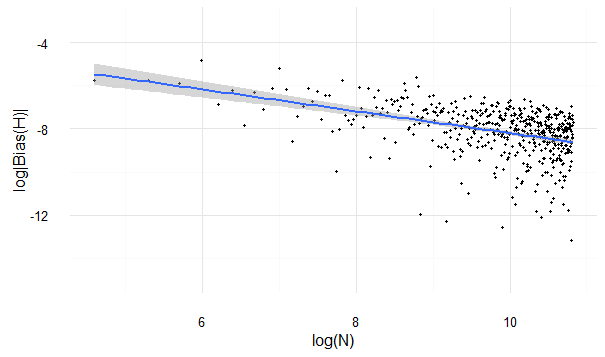
\includegraphics[width=\textwidth]{./Graphs/Best/Normal_k=1.png}\label{normal_k=1}
\caption{k=1}
\end{subfigure}%
\begin{subfigure}[b]{.8\textwidth}
\centering
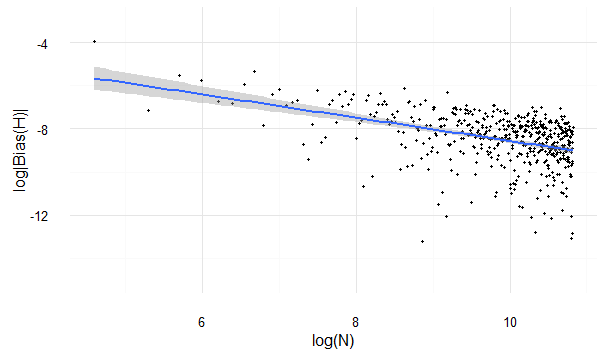
\includegraphics[width=\textwidth]{./Graphs/Best/Normal_k=2.png}\label{normal_k=2}
\caption{k=2}
\end{subfigure}%
}\    \makebox[\linewidth][c]{%
\begin{subfigure}[b]{.8\textwidth}
\centering
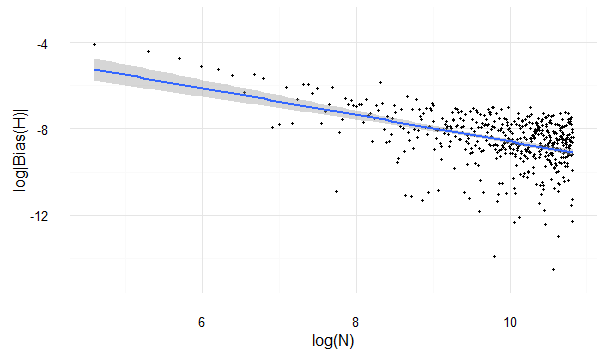
\includegraphics[width=\textwidth]{./Graphs/Best/Normal_k=3.png}\label{normal_k=3}
\caption{k=3}
\end{subfigure}%
\begin{subfigure}[b]{.8\textwidth}
\centering
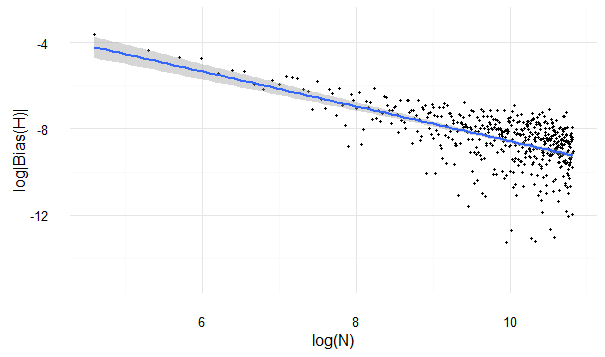
\includegraphics[width=\textwidth]{./Graphs/Best/Normal_k=4.png}\label{normal_k=4}
\caption{k=4}
\end{subfigure}%
}\    \makebox[\linewidth][c]{%
\begin{subfigure}[b]{.8\textwidth}
\centering
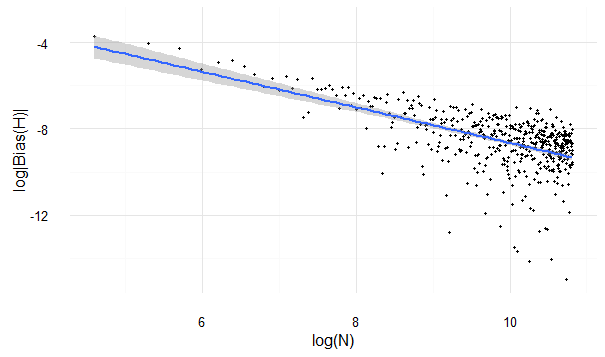
\includegraphics[width=\textwidth]{./Graphs/Best/Normal_k=5.png}\label{normal_k=5}
\caption{k=5}
\end{subfigure}%
\begin{subfigure}[b]{.8\textwidth}
\centering
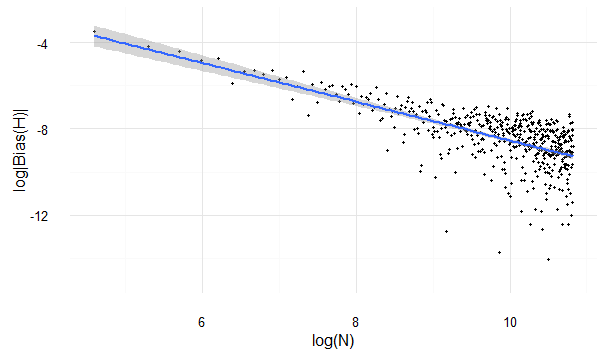
\includegraphics[width=\textwidth]{./Graphs/Best/Normal_k=6.png}\label{normal_k=6}
\caption{k=6}
\end{subfigure}%
}
\caption{1-dimensional normal distribution with different $k = 1, ..., 6$} \label{normal_graphs16}
\end{figure}


\begin{figure}
\makebox[\linewidth][c]{%
\begin{subfigure}[b]{.8\textwidth}
\centering
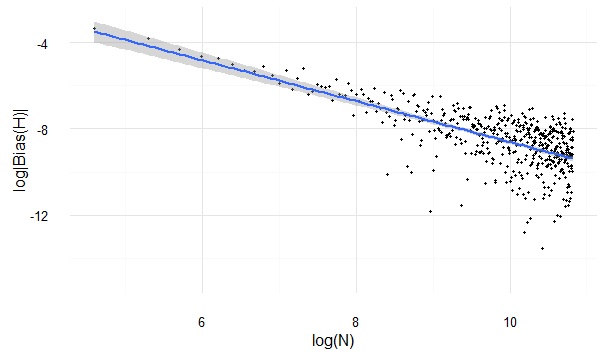
\includegraphics[width=\textwidth]{./Graphs/Best/Normal_k=7.png}\label{normal_k=7}
\caption{k=7}
\end{subfigure}%
\begin{subfigure}[b]{.8\textwidth}
\centering
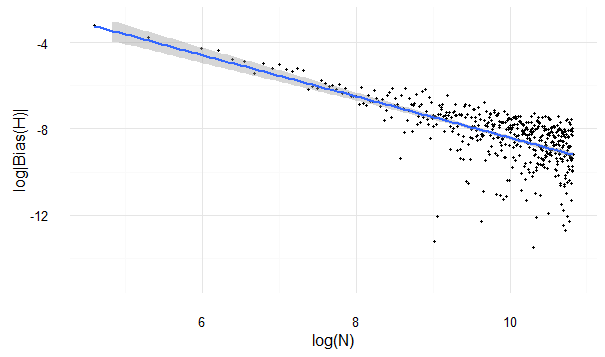
\includegraphics[width=\textwidth]{./Graphs/Best/Normal_k=8.png}\label{normal_k=8}
\caption{k=8}
\end{subfigure}%
}\    \makebox[\linewidth][c]{%
\begin{subfigure}[b]{.8\textwidth}
\centering
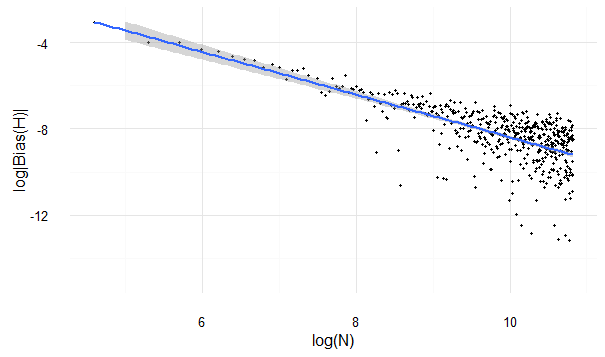
\includegraphics[width=\textwidth]{./Graphs/Best/Normal_k=9.png}\label{normal_k=9}
\caption{k=9}
\end{subfigure}%
\begin{subfigure}[b]{.8\textwidth}
\centering
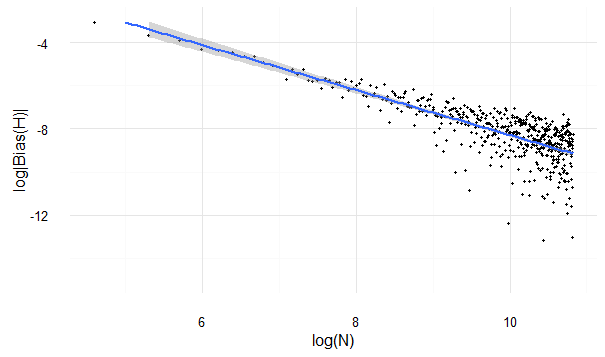
\includegraphics[width=\textwidth]{./Graphs/Best/Normal_k=10.png}\label{normal_k=10}
\caption{k=10}
\end{subfigure}%
}\    \makebox[\linewidth][c]{%
\begin{subfigure}[b]{.8\textwidth}
\centering
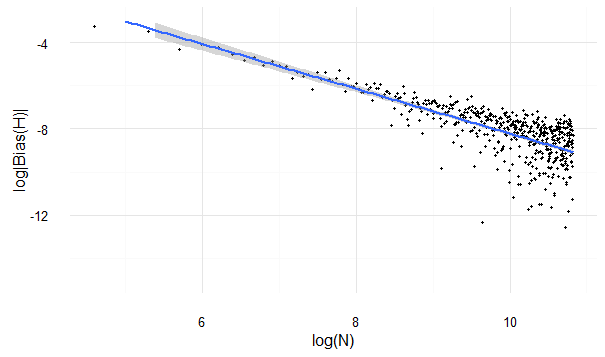
\includegraphics[width=\textwidth]{./Graphs/Best/Normal_k=11.png}\label{normal_k=11}
\caption{k=11}
\end{subfigure}%
}
\caption{1-dimensional normal distribution with different $k = 7, ...,11$} \label{normal_graphs711}
\end{figure}

Moreover, I would like to consider the coefficient of determination ($R^2$) for each of the above regression lines, this value provides an estimate of the strength of the relationship between the model and the response variable. Also, I would like to consider the standard error/deviation ($\sigma$), for each of the different graphs, which shows a measure of the predictions' accuracy. These are all depicted for each value of $k$ in table \ref{normal_rsq}.

\begin{table}
\caption{Comparison of the coefficient of determination and the standard deviations of the regression for each value of $k$ for the 1-dimensional normal distribution} \label{normal_rsq}
\begin{center}
\begin{tabular}{| l | c c |} 
\toprule
$k$ & $R^2$ & $\sigma$ \\
\midrule[1pt]
1     & 0.1766    & 1.0661    \\
2     & 0.1793    & 1.1477    \\
3     & 0.2292    & 1.1053    \\
4     & 0.3556    & 1.0759    \\
5     & 0.3322    & 1.1752   \\
6     & 0.4260    & 1.0180   \\
7     & 0.4532    & 1.0155   \\
8     & 0.4623    & 1.0088   \\
9     & 0.4962    & 0.9730   \\
10    & 0.5227    & 0.9759   \\
11    & 0.5839    & 0.8566  \\
\hline
\end{tabular}
\\[10pt]
\end{center}
\end{table}

Both columns of this table essentially point to the same conclusion; the larger the value of $k$, the more accurate the linear model is to fitting the data. This is shown by the $R^2$ value increasing towards $1$ and the $\sigma$ values decreasing positively. 

The $R^2$ is very small for $k \leq 3$ , which points towards the line being a poor fir to the data; however, due the the standard deviation being $\sigma^2 \approx 1.1$, we cannot say that these lines are poorly fitting; since the majoring of the data is within a very small range of the line.

The most important information found from the regression analysis is shown in table \ref{normal_a_c_compare_table}; where the values of $a_{k}$ and $c_{k}$ are given for each value of $k$.

\begin{table}
\caption{Comparison of coefficients of regression $a_{k}$ and $c_{k}$ from equation \ref{bias}, for 1-dimensional normal distribution} \label{normal_a_c_compare_table}
\begin{center}
\begin{tabular}{| l | l l |} 
\toprule
$k$ &  $a_{k}$ & $c_{k}$ \\
\midrule[1pt]
1  &  0.5054 & 0.0433 \\
2  & 0.5490 & 0.0459 \\
3  & 0.6169 & 0.0894 \\
4  & 0.8181 & 0.6690 \\
5  & 0.8486 & 0.8235 \\
6  & 0.8976 & 1.5514 \\
7  & 0.9464 & 2.3576 \\
8  & 0.9574 & 3.2021 \\
9  & 0.9883 & 4.4558 \\
10 & 1.0454 & 8.5402 \\
11 & 1.0386 & 8.7457 \\
\hline
\end{tabular}
\\[10pt]
\end{center}
\end{table}

As $k$ runs from $1 \to 11$, we have that $a_{k}$ and $c_{k}$ both increase, with smooth values of $a_{k}$ and a large jump, in the value of $c_{k}$, between $k=3$ and $4$, and $k=9$ and $10$. The higher the value of $a_{k}$, the stronger the negative relationship is between the two variables in question, so for a larger values of $a_{k}$, we have that $|Bias(\hat{H}_{N, k})| \to 0$ for large $N$ faster than smaller values of $a_{k}$. This is due to the relationship between $|Bias(\hat{H}_{N, k})|$ and $a_{k}$ shown in equation (\ref{bias})

Recall, from section \ref{focus} we have that the bias acts in one of two ways (equations \ref{fixedkbias} and \ref{dependentkbias}); it is either of $O \left( \frac{1}{N^{a}} \right)$ or $O\left( \left( \frac{k}{N} \right)^{a} \right)$. Thus we have $|Bias(\hat{H}_{N, k})|\approx \frac{c_{k}}{N^{a_{k}}}$ where either $c_{k}$ is constant or it depends on $k$ and $a_{k}$ - more specifically is $O( k^{a_{k}})$. There is evidence here to support the latter claim. If we consider the jump between $k=3$ and $4$ shown in the value of $c_{k}$, and consider the results in table \ref{normal_dependentk}. 

\begin{table}
\caption{Considering the dependence of $k$ on $c_{k}$} \label{normal_dependentk}
\begin{center}
\begin{tabular}{| l | l l l |} 
\toprule
$k$ &  $k^{a_{k}}$ & $c_{k}$ & $\frac{k^{a_{k}}}{c_{k}}$ \\
\midrule[1pt]
1  & 1 & 0.0433 & 23.095 \\
2  & 1.4631 & 0.0459 & 31.875 \\
3  & 1.9694 & 0.0894 & 22.029 \\
4  & 3.1085 & 0.6690 & 4.646 \\
5  & 3.9187 & 0.8235 & 4.759 \\
6  & 4.9942 & 1.5514 & 3.219 \\
7  & 6.3067 & 2.3576 & 2.675 \\
8  & 7.3218 & 3.2021 & 2.287 \\
9  & 8.7716 & 4.4558 & 1.969 \\
10 & 11.1020 & 8.5402 & 1.300 \\
11 & 12.0668 & 8.7457 & 1.380 \\
\hline
\end{tabular}
\\[10pt]
\end{center}
\end{table}

This shows that the proportional behaviour between $k^{a_{k}}$ and $c_{k}$ also has a large jump when $k$ goes from $3 \to 4$. This agrees with the claim of $c_{k}$ depending on $k$ in this fashion; however, in table \ref{normal_a_c_compare_table} we mentioned another jump between $k=9$ and $k=10$, and the evidence here does not show a large jump in the same area. We cannot yet make any conclusions about the dependence of $c_{k}$ on $k$; this motivates a graphical representation of the value of $c_{k}$ against $k$ to see if there is any relation, Figure \ref{c_k_normal}.

\begin{figure}
\makebox[\linewidth][c]{%
\begin{subfigure}[b]{.8\textwidth}
\centering
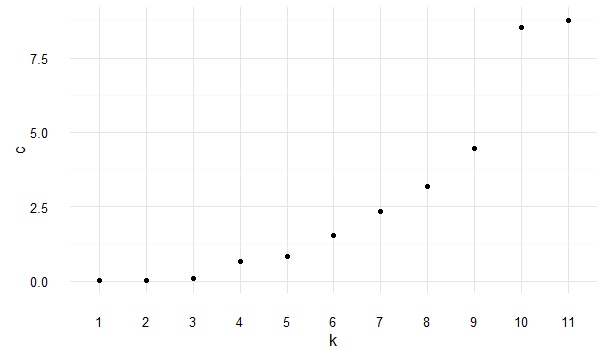
\includegraphics[width=\textwidth]{./Graphs/Best/NormalcVk.png}
\caption{The values of $k$ against the values of $c_{k}$}
\end{subfigure}%
\begin{subfigure}[b]{.8\textwidth}
\centering
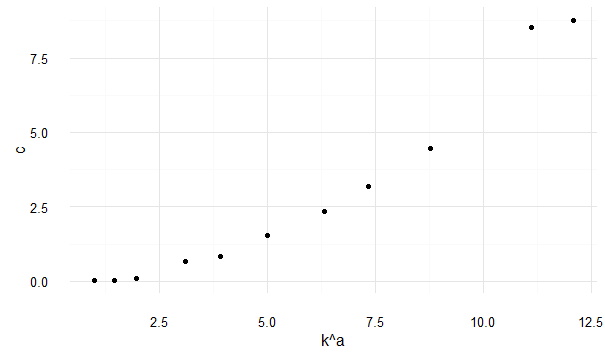
\includegraphics[width=\textwidth]{./Graphs/Best/NormalcVk2.png}
\caption{The values of $k^{a_{k}}$ against the corresponding values of $c_{k}$}
\end{subfigure}%
}
\caption{Graphically representing the relationship between $c_{k}$ and $k$} \label{c_k_normal}
\end{figure}

Interestingly, plot \ref{c_k_normal} (a) shows an almost exponential relationship between the values of $c_{k}$ and the values of $k$. This leads me to believe that there is some kind of relationship between the two variables, and looking at plot \ref{c_k_normal}(b) this shows that there's a strong possibility that the relationship is of the form stated in equation \ref{dependentkbias}.

To better study the linear relationship between the logarithm of the bias and the logarithm of the sample size, I have generated a comparison plot, shown in Figure \ref{normal_comparison_graph}. 

\begin{figure}
  \begin{center}
    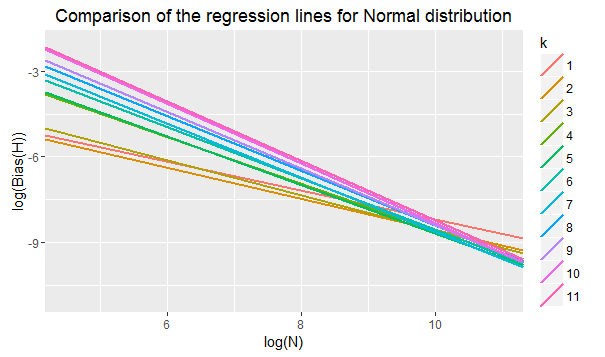
\includegraphics[width=\textwidth]{./Graphs/Best/NormalComparison.png}
  \end{center}
\caption{Plot of regression lines for $\log|Bias(\hat{H}_{N, k})|$ against $\log(N)$, for $k=1, 2,..., 11$, for samples from the normal distribution}
  \label{normal_comparison_graph}
\end{figure}

From this we can see obviously that for smaller values of $N$, smaller values of $log(N)$, the smallest bias occurs when $k=2$, since this line is the lowest for the data up until $log(N) \approx 9$ - i.e. $N \approx 13,000$. For a larger sample size, we cannot accurately see in this graph which line is the best. This motivates us to look at a section of the graph when $9 \leq log(N) \leq 11$ - i.e. $8,000 \leq N \leq 50,000$, which is shown in Figure \ref{normal_comparison_graph_zoom}.

\begin{figure}
  \begin{center}
    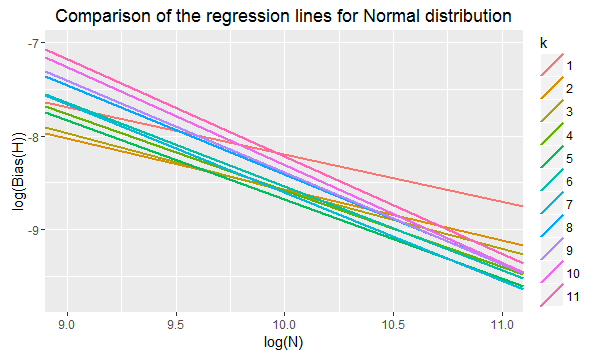
\includegraphics[width=\textwidth]{./Graphs/Best/NormalComparisonZoom.png}
  \end{center}
\caption{Figure \ref{normal_comparison_graph} zoomed in around large $N$}
  \label{normal_comparison_graph_zoom}
\end{figure}

From this graph we can obviously discount $k=1$ for large $N$, since this is the most gradual descent; thus the bias will be largest for this $k$. Also, both the lines for $k=2$ and $k=3$ are more gradual in their descent at larger $N$, so are probably not the best to choose. Even though, for $k=9, 10$ and $11$, the slope is the steepest - $a_{k}$ is largest - the intercept is larger so around the biggest sample size considered $N=50,000$, $log(N) \approx 10.8$, there is not the smallest bias. Actually, for large values of $N \leq 50,000$ we can see from this graph that the best lines appear to be those which are blue/green; $k = 4, 5, 6, 7, 8$. Where the lowest lines around the maximal sample size are those for $k=5$ and $k=7$; thus these values of $k$ could possible be the best nearest neighbour value to choose, when looking at a sample of size $N \approx 50,000$ from the normal distribution.











\section{1-dimensional Uniform Distribution} \label{Uniform_d=1}

I will now explore the entropy of samples from the 1-dimensional uniform distribution, $U[a, b]$. This distribution also has an exact formula to work out the entropy for. We can find this formula by considering the density function, $f$, from the uniform distribution, which is given by;
\[
f(x) =  \begin{cases} 
      \frac{1}{b-a} & a \leq x \leq b \\
      0 & otherwise
   \end{cases}
\]
Using the definition of Shannon entropy given in equation (\ref{ShaEnt}), we can find the exact entropy for the uniform distribution;
\begin{align*}
H &= - \int_{x \in \mathbb{R}^d} f(x) log(f(x)) dx \\ 
&= - \int_{a}^{b} \frac{1}{b-a} log \left[ \frac{1}{b-a} \right] dx  \\
&= - \frac{1}{b-a} log \left[ \frac{1}{b-a} \right]  \int_{a}^{b} dx  \\
&= -  log  \left[ \frac{1}{b-a} \right] 
\end{align*}
Thus, the actual value of entropy for the uniform distribution is given by;
\begin{equation} \label{UnifEnt}
H = log [ b-a ]
\end{equation}

Similarly to the 1-dimensional normal distribution, we have for the 1-dimensional uniform distribution that $d=1$ so $V_{1} = 2$, thus our estimator takes the form of equation (\ref{KLest_d=1});
\begin{equation}
\hat{H}_{N, k} =  \frac{1}{N} \sum_{i=1}^{N} log \left[ \frac{2\rho_{(k),i}(N-1)}{e^{\Psi(k)}} \right]\nonumber
\end{equation}

Moreover, the samples considered will not be from the standard uniform, but from the uniform distribution $U[0,100]$. This is because, using the standard uniform, $U[0,1]$, would fail since taking $N=50,000$ samples between 0 and 1 would generate problems as the density function would be $f(x) = 1 , \quad 0 \leq x \leq 1$, which would incur working on a very small scale; i.e taking a points with distance between them. Thus, I will be using the density function $f(x) = 0.01$, $0 \leq x \leq 100$, which is from the $U[0,100]$ distribution and gives the exact entropy to be;
\begin{equation} \label{uniform_exact}
H = log(100) \approx 4.605170
\end{equation}




\subsection{Estimator Conditions} \label{U_Conditions}

For Theorems \ref{unbias} and \ref{efficient} to be satisfied by the estimators generated by samples from the uniform distribution, this density function must meet the Conditions \ref{A1}, \ref{A2} and \ref{A3}. 
Firstly, to satisfy Condition \ref{A1}, for the density function $f(x) = 0.01$ for $0 \leq x \leq 100$, it must be such that;
\begin{itemize}
\item f is bounded - obviously, since the density function for the uniform distribution is constant for $x \in [a, b]$ and $0$ otherwise; hence is bounded.

\item f is m-times differentiable - as $f$ is constant this holds

\item $\exists r_{*} > 0$ and a Borel measurable function $g_{*}$, with $\|y-x\| \leq r_{*}$ so that $\|f^{(t)}(x)\| \leq g_{*}(x) f(x)$ and $\|f^{(m)}(x) - f^{(m)}(x)\| \leq g_{*}(x) f(x)\|y - x\|^{\eta}$, for some $g_{*}$ such that $\sup_{\{x : f(x) < \delta\}} g_{*}(x) = O(\delta^{-\epsilon})$ as $\delta \searrow 0$ for some $\epsilon >0$.
This is elementary since $f$ is constant, thus $f^{(t)}(x) = 0$ for all $t \geq 1$, so we can always fins an appropriate $g_{*}(x)$.

\end{itemize}

Next, to satisfy Condition \ref{A2}, for the density function $f$ of the uniform distribution, must fulfill that;
\begin{itemize}
\item The $\alpha$-moment of $f$ must be finite, so $\int_{\mathbb{R}^{d}} \| x \|^{\alpha} f(x) dx < \infty$ - this is true, since for the 1-dimensional uniform distribution, $f(x)$ is constant; thus we would be integrating a polynomial $|x|^{\alpha}$, over a finite interval $a \leq x \leq b$, which is always finite.
\end{itemize}

Lastly, to satisfy Condition \ref{A3}, we must find the values of $k$ for which the estimator provides a uniform convergence for Theorems \ref{unbias} and \ref{efficient}. These values are independent of the distribution that the sample is from, and only depends on the size of the sample, the dimension of the distribution that sample is taken from and the value chosen for $\alpha$, where we have chosen $\alpha = 2$. The values of $k$ found in section \ref{N_conditions} are $\{1,2\}$ for $N=100$, $\{1, 2, ..., 9\}$ for $N=25,000$ and then $\{1, 2, ..., 11\}$ for $N=50,000$. 

Thus, due to the above conditions for Theorems \ref{unbias} and \ref{efficient} being met, we can say that the Kozachenko-Leonenko estimator, of a sample from the uniform distribution is an asymptotically unbiased and consistent estimator for entropy, for specific $k \in \{1, 2, ..., 11 \}$, depending on the sample size $N$.




\subsection{Simulation Results} \label{Uniform_results}

I will now conduct simulations, in a similar manner as for the normal distribution, where for each value of $k$ separately, I will consider $500$ samples of size $N$ from the uniform distribution, finding the estimator in each case and take the average of these estimators to find our entropy estimator. I will then consider the relationship show in equation (\ref{logbias}) for each sample and work out the average for the values of a and c, for each $k \in \{1, 2, ..., 11\}$. 

For $N=100$, $N=25,000$ and $N=50,000$, using the results from \ref{appendix_data}, we can create a table to compare the mean values of the bias of the estimator for the different values of $k$ considered. 

\begin{table}
\caption{1-dimensional uniform distribution, comparison of $k$} \label{uniform_kcompare_table}
\begin{center}
\begin{tabular}{| l | c c c |} 
\toprule
$k$ &  $|Bias(\hat{H}_{100, k})|$ & $|Bias(\hat{H}_{25000, k})|$  &  $|Bias(\hat{H}_{50000, k})|$ \\
\midrule[1pt]
1     & 0.0005189    &       Inf    &       Inf   \\
2     & 0.0047466    & 0.0001745    & 0.0001163   \\
3     & 0.0083912    & 0.0001776    & 0.0000899   \\
4     & 0.0169364    & 0.0001177    & 0.0000490   \\
5     & 0.0152168    & 0.0000588    & 0.0000509   \\
6     & 0.0148205    & 0.0000817    & 0.0000538   \\
7     & 0.0218339    & 0.0002918    & 0.0000663   \\
8     & 0.0250401    & 0.0001884    & 0.0000487   \\
9     & 0.0297655    & 0.0001406    & 0.0001184   \\
10    & 0.0337164    & 0.0001337    & 0.0000949   \\
11    & 0.0381473    & 0.0001693    & 0.0000417   \\
\hline
\end{tabular}
\\[10pt]
\caption*{This table is comparing the values of $|Bias(\hat{H}_{N, k})|$ for the values of $k$ with $N=100$, $N=25,000$ and $N=50,000$, when the estimator is taken over $500$ samples}
\end{center}
\end{table}

Looking at the results shown in table \ref{uniform_kcompare_table}, for $N=100$, we can see that the smallest bias, quite obviously, occurs when the estimator is taken with $k=1$, and that for other values of $k$ there is a significant difference in the size of the bias.

When looking at the larger values of $N$, it is first important to note that \texttt{Inf} $= \infty$ is present in the table as for a large value of $N$, it is difficult to work out the estimator when $k=1$. This is because there are only extremely small distances between the closest samples of this distribution, and since any program used to compute these numbers will fail with extremely small numbers and default them to \texttt{- Inf}. We only need there to be two samples with an infinitely small distance to make the whole estimator become \texttt{- Inf}, which is \texttt{Inf} when looking at the modulus. This was mentioned earlier and was the motivation for taking the uniform distribution over $[0, 100]$; however, because of this, from now onwards I will not be considering $k=1$ in the estimator for the uniform distribution.

Thus, looking at the results shown in table \ref{uniform_kcompare_table}, ignoring $k=1$ and considering $N=25,000$, it appears to show smallest bias for values of $k \in \{4, 5, 6 \}$; more specifically $k=5$ appears to have the smallest bias. This fits with the previous analysis done on the value of $k$ for different sample sizes, which stated that we must have $k \in \{1, 2, ..., 9\}$. Next, examining the table for $N=50,000$, we can see that the smallest bias looks to be when $k \in \{ 4, 5, 6, 7, 8, 11\}$, however, for all other values of $k$ we still have a small bias $< 0.000012$. Thus, we cannot yet draw any conclusions about the optimal value of $k$ for large $N$ and this distribution.

Next I wish to examine the graphs showing the relationship in equation \ref{logbias}, by plotting the simulated data and fitting a regression line for each value of $k$ separately, in figures \ref{Uniform_graphs26} and \ref{Uniform_graphs711}. Thus showing a negative linear relationship between the logarithm of the bias of the estimator and the logarithm of the sample size $N$. Also, looking more closely, the regression lines fitted to the data appear to become more steep for higher values of $k$, whilst the standard error bars appear to become smaller. 

\begin{figure}
\makebox[\linewidth][c]{%
\begin{subfigure}[b]{.8\textwidth}
\centering
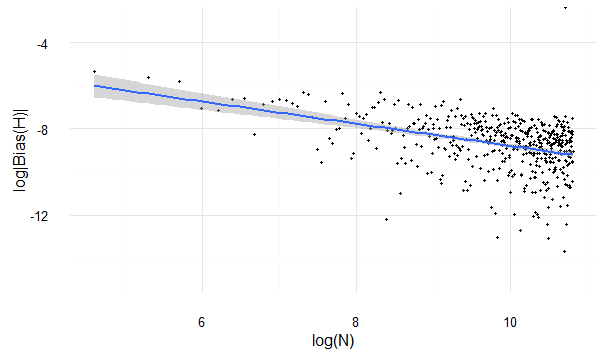
\includegraphics[width=\textwidth]{./Graphs/Best/Uniform_k=2.png}
\caption{k=2}
\end{subfigure}%
\begin{subfigure}[b]{.8\textwidth}
\centering
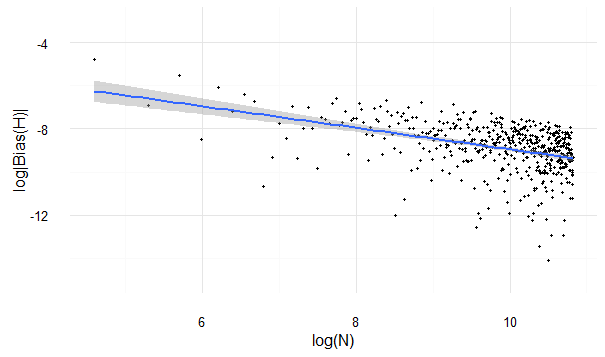
\includegraphics[width=\textwidth]{./Graphs/Best/Uniform_k=3.png}
\caption{k=3}
\end{subfigure}%
}\    \makebox[\linewidth][c]{%
\begin{subfigure}[b]{.8\textwidth}
\centering
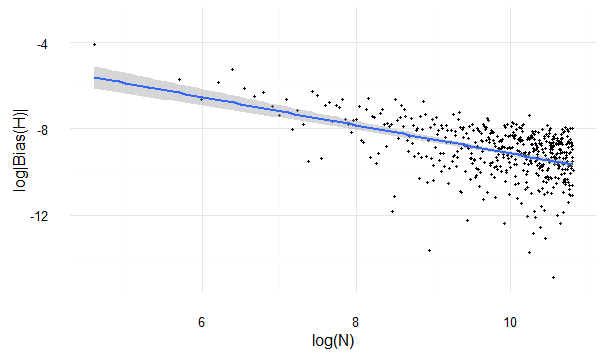
\includegraphics[width=\textwidth]{./Graphs/Best/Uniform_k=4.png}
\caption{k=4}
\end{subfigure}%
\begin{subfigure}[b]{.8\textwidth}
\centering
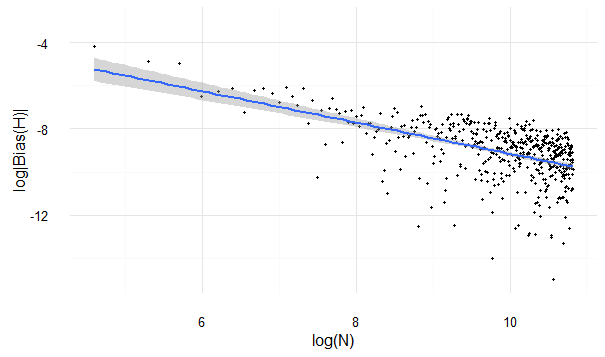
\includegraphics[width=\textwidth]{./Graphs/Best/Uniform_k=5.png}
\caption{k=5}
\end{subfigure}%
}\    \makebox[\linewidth][c]{%
\begin{subfigure}[b]{.8\textwidth}
\centering
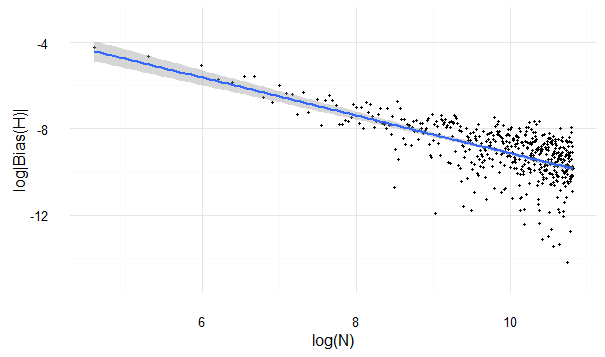
\includegraphics[width=\textwidth]{./Graphs/Best/Uniform_k=6.png}
\caption{k=6}
\end{subfigure}%
}
\caption{1-dimensional Uniform distribution with different $k = 2, ..., 6$} \label{Uniform_graphs26}
\end{figure}


\begin{figure}
\makebox[\linewidth][c]{%
\begin{subfigure}[b]{.8\textwidth}
\centering
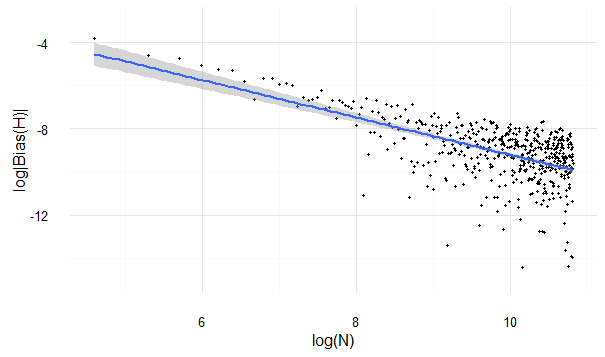
\includegraphics[width=\textwidth]{./Graphs/Best/Uniform_k=7.png}
\caption{k=7}
\end{subfigure}%
\begin{subfigure}[b]{.8\textwidth}
\centering
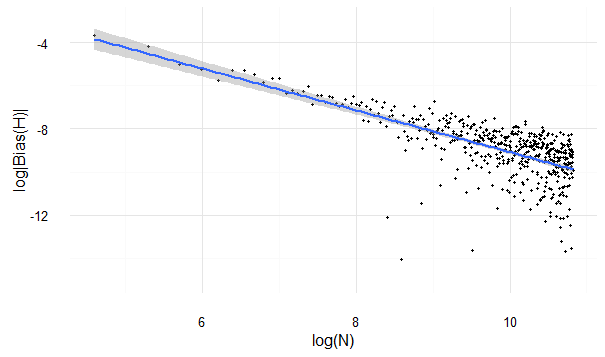
\includegraphics[width=\textwidth]{./Graphs/Best/Uniform_k=8.png}
\caption{k=8}
\end{subfigure}%
}\    \makebox[\linewidth][c]{%
\begin{subfigure}[b]{.8\textwidth}
\centering
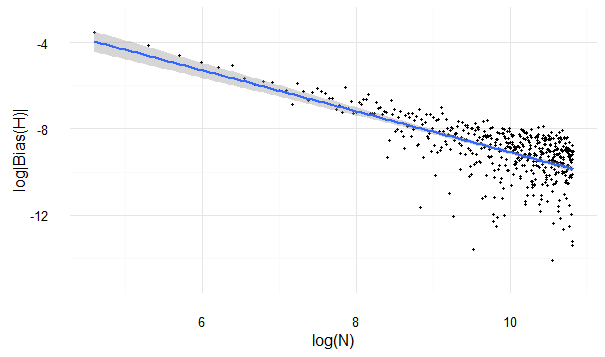
\includegraphics[width=\textwidth]{./Graphs/Best/Uniform_k=9.png}
\caption{k=9}
\end{subfigure}%
\begin{subfigure}[b]{.8\textwidth}
\centering
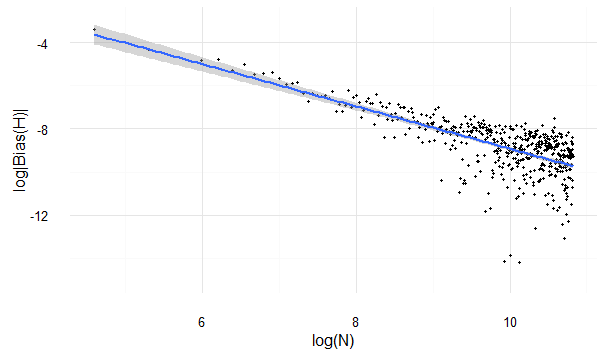
\includegraphics[width=\textwidth]{./Graphs/Best/Uniform_k=10.png}
\caption{k=10}
\end{subfigure}%
}\    \makebox[\linewidth][c]{%
\begin{subfigure}[b]{.8\textwidth}
\centering
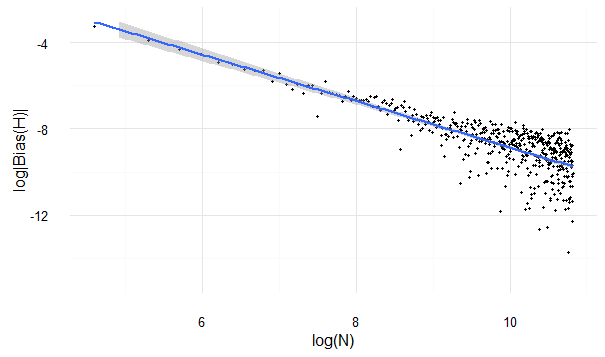
\includegraphics[width=\textwidth]{./Graphs/Best/Uniform_k=11.png}
\caption{k=11}
\end{subfigure}%
}
\caption{1-dimensional Uniform distribution with different $k = 7, ..., 11 $} \label{Uniform_graphs711}
\end{figure}

Another important thing to consider, before looking at the equations of the regression lines, is to see how well these lines actually fit the data. To do this I have, as before, examined the coefficient of determination and the standard deviation of the lines, Table \ref{uniform_rsq}.

\begin{table}
\caption{Comparison of the coefficient of determination and the standard deviations of the regression for each value of $k$ for the 1-dimensional uniform distribution} \label{uniform_rsq}
\begin{center}
\begin{tabular}{| l | c c |} 
\toprule
$k$ & $R^2$ & $\sigma$ \\
\midrule[1pt]
2     & 0.1721    & 1.0982   \\
3     & 0.1576    & 1.1402   \\
4     & 0.2485    & 1.1200   \\
5     & 0.2784    & 1.1459   \\
6     & 0.4027    & 1.0286   \\
7     & 0.3605    & 1.1252   \\
8     & 0.4689    & 1.0073   \\
9     & 0.4653    & 0.9940   \\
10    & 0.5088    & 0.9408   \\
11    & 0.6215    & 0.8208   \\
\hline
\end{tabular}
\\[10pt]
\end{center}
\end{table}

This table is very similar to that for the normal distribution in that both columns point towards the same conclusion; the larger that $k$ is, the more accurate the linear model is to fitting the data. This is shown by the $R^2$ value generally increasing towards $1$ and the $\sigma$ values decreasing positively - the deviation about the line is decreasing for higher $k$. There is slight fluctuation in the middle values of $k$, where for $k = \{6, 7, 8\}$ there is not an exact direction that the relationship is going. However, there is nothing to say that this isn't normal behaviour, since we do not yet know the relationship between the bias and $k$.

Moreover, $R^2$ is very small for $k \leq 4$ , which points towards the line being a poor fir to the data; however, due the the standard deviation being $\sigma \approx 1.1$, we cannot discard the importance of these lines; since most of the data is in a very small range about the line. Additionally, for $k=11$ we have the strongest relationship seen so far - the largest $R^2$ and smallest $\sigma$ values appear - this could indicate that for this distribution, when $k=11$ the linear relationship between the logarithm of the bias and the logarithm of the sample size is most likely to be true.

Possibly the most important information found from the regression analysis, is shown in Table \ref{uniform_a_c_compare_table}; where the values of $a_{k}$ and $c_{k}$ are given for each value of $k = \{ 2, 3, ..., 11\}$.

\begin{table}
\caption{Comparison of coefficients of regression $a_{k}$ and $c_{k}$ from equation \ref{bias}, for 1-dimensional uniform distribution} \label{uniform_a_c_compare_table}
\begin{center}
\begin{tabular}{| l | l l |} 
\toprule
$k$ &  $a_{k}$ & $c_{k}$ \\
\midrule[1pt]
2     & 0.5125    & 0.0258   \\
3     & 0.5048    & 0.0199   \\
4     & 0.6593    & 0.0779   \\
5     & 0.7286    & 0.1531   \\
6     & 0.8645    & 0.6090   \\
7     & 0.8648    & 0.5758   \\
8     & 0.9688    & 1.8377   \\
9     & 0.9492    & 1.5095   \\
10    & 0.9801    & 2.4041   \\
11    & 1.0765    & 6.6932   \\
\hline
\end{tabular}
\\[10pt]
\end{center}
\end{table}

We wish to have a value of $a_{k} \geq 0.5$ to show the relationship desired, and this is true for all values of $k$ in this table. As $k$ increases, we have that both $a_{k}$ and $c_{k}$ increase, expect for $k=8$, which has larger values that $k=9$. However, this slight change around $k=8$ does not necessarily imply anything dramatic since the overall trend seems to fit with that found for the normal distribution.

To better see if the relationship of the bias of the estimator and the sample size is of the form of equations \ref{fixedkbias} and \ref{dependentkbias}; either $O \left( \frac{1}{N^{a}} \right)$ or $O\left( \left( \frac{k}{N} \right)^{a} \right)$. Thus I will consider the value of $c_{k}$ for each $k$, to see if it is dependent on $k^a_{k}$ or not, shown in table \ref{uniform_dependentk}.

\begin{table}
\caption{Considering the dependence of $k$ on $c_{k}$} \label{uniform_dependentk}
\begin{center}
\begin{tabular}{| l | l l l |} 
\toprule
$k$ &  $k^{a_{k}}$ & $c_{k}$ & $\frac{k^{a_{k}}}{c_{k}}$ \\
\midrule[1pt]
2     &  1.4265    & 0.0258    &    55.291   \\
3     &  1.7412    & 0.0199    &    87.498   \\
4     &  2.4942    & 0.0779    &    32.019   \\
5     &  3.2305    & 0.1531    &    21.101   \\
6     &  4.7066    & 0.6090    &     7.729   \\
7     &  5.3807    & 0.5758    &     9.345   \\
8     &  7.4975    & 1.8377    &     4.080   \\
9     &  8.0495    & 1.5095    &     5.332   \\
10    &  9.5521    & 2.4041    &     3.973   \\
11    & 13.2148    & 6.6932    &     1.974   \\
\hline
\end{tabular}
\\[10pt]
\end{center}
\end{table}

This shows that the proportional behaviour between $k^{a_{k}}$ and $c_{k}$ does not imply that $c_{k} = O(k^a_{k})$, since there is no exact trend in the numbers, other than a slight decrease as $k$ increases. However, this increase is not uniform so we can make little assumptions about the behaviour of $c_{k}$, perhaps a better way to show this relationship is through a graphical representation of $c_{k}$ against $k$ to see what form it takes.

\begin{figure}
\makebox[\linewidth][c]{%
\begin{subfigure}[b]{.8\textwidth}
\centering
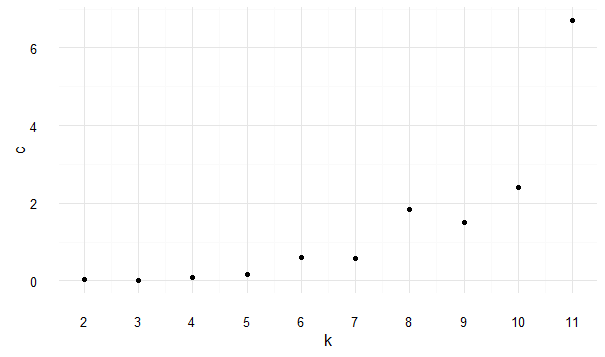
\includegraphics[width=\textwidth]{./Graphs/Best/UniformcVk.png}
\caption{The values of $k$ against the values of $c_{k}$}
\end{subfigure}%
\begin{subfigure}[b]{.8\textwidth}
\centering
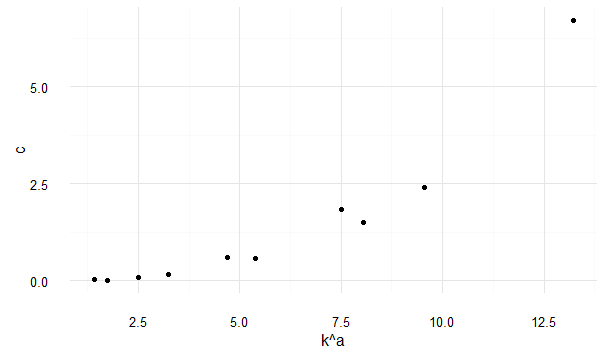
\includegraphics[width=\textwidth]{./Graphs/Best/UniformcVk2.png}
\caption{The values of $k^{a_{k}}$ against the corresponding values of $c_{k}$}
\end{subfigure}%
}
\caption{Graphically representing the relationship between $c_{k}$ and $k$ for the uniform distribution} \label{c_k_uniform}
\end{figure}

Figure \ref{c_k_uniform}, for the uniform distribution tells a slightly different story to that of the normal. It does seem to show an almost exponential relationship, as before, however, there are a larger number of outlier values that do not fit within a smooth line in these graphs than in those for the normal distribution, Figure \ref{c_k_normal}. However, the relationship that is shown leads me to believe that there is something important between the two variables, which could possibly be of the form stated in equation \ref{dependentkbias}.

To better study the linear relationship between the logarithm of the bias and the logarithm of the sample size, I have generated a comparison plot, shown in Figure \ref{normal_comparison_graph}. 

\begin{figure}
  \begin{center}
    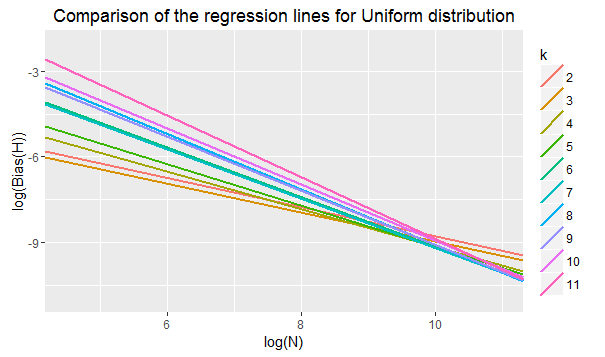
\includegraphics[width=\textwidth]{./Graphs/Best/UniformComparison.png}
  \end{center}
\caption{Plot of regression lines for $\log|Bias(\hat{H}_{N, k})|$ against $\log(N)$, for $k=2, 3,..., 11$, for samples from the uniform distribution}
  \label{uniform_comparison_graph}
\end{figure}

For the smaller values of $N$, when $N \approx 100$, we can see obviously from this plot that the lowest line occurs from $k=3$, and this value of $k$ stays the best for the estimator until $log(N) \approx 8.5$, so the sample size $N \approx 5,000$. Above this value, it appears to be that the smallest bias occurs from when $k \in \{7, 8, 9, 11\}$, to see this more accurately consider an enlarged version of this graph for $5,000 < N < 50,000$, Figure \ref{uniform_comparison_graph_zoom}.

\begin{figure}
  \begin{center}
    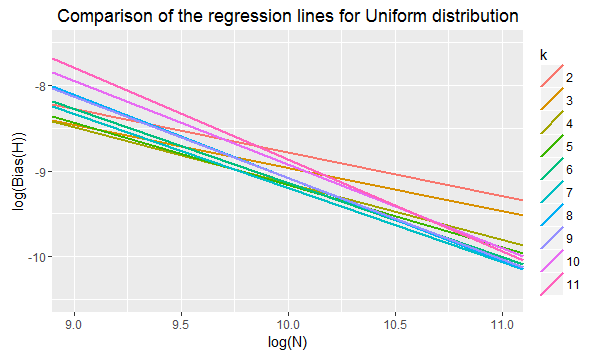
\includegraphics[width=\textwidth]{./Graphs/Best/UniformComparisonZoom.png}
  \end{center}
\caption{Figure \ref{uniform_comparison_graph} zoomed in around large $N$.}
  \label{uniform_comparison_graph_zoom}
\end{figure}

This graph shows that for large $N \leq 50,000$, the lowest line on the graph is when the estimator is found using $k=7$; thus there is a possibility that this value of $k$ could be the best nearest neighbour value to choose, when considering sample size $N \approx 50,000$ from the uniform distribution.









\section{1-dimensional Exponential Distribution} \label{Expo_d=1}

I will now be looking at the entropy of samples from the exponential distribution $exp(\lambda)$, where $\lambda > 0$ is the rate or inverse scale parameter. In a similar fashion to the previous distributions, the exponential also has an exact formula for the entropy, given the rate parameter $\lambda$. Using equation (\ref{ShaEnt}) and the density function for the exponential distribution $f(x) = \lambda e^{-\lambda x}$ for $x \in [0, \infty)$ and for $\lambda >0$, we can write the exact entropy;
\begin{align*}
H &= - \int_{x \in \mathbb{R}^d} f(x) log(f(x)) dx \\ 
&= - \int_{0}^{\infty} \lambda e^{-\lambda x} log [ \lambda e^{-\lambda x} ] dx  \\
&= - \lambda \int_{0}^{\infty} \lambda e^{-\lambda x} [log(\lambda) - \lambda x] dx  \\
&= \lambda \int_{0}^{\infty} \lambda e^{-\lambda x} - log(\lambda) e^{-\lambda x} dx \\
&= - \lambda \left[x e^{-\lambda x}\right]_{0}^{\infty} + \int_{0}^{\infty}\lambda e^{-\lambda x} dx + log(\lambda) \left[ e^{-\lambda x}\right]_{0}^{\infty} \\
&= 0 + (log(\lambda) - 1) \left[e^{-\lambda x} \right]_{0}^{\infty} \\
&= -(log(\lambda) - 1)
\end{align*}

Thus we have the the exact value of entropy for the exponential distribution, given the rate parameter $\lambda > 0$, is;
\begin{equation} \label{ExpEnt}
H = 1 - log(\lambda)
\end{equation}

Moreover, I am again considering a 1-dimensional distribution; thus $V_{d} = V_{1} = 2$, and;
\begin{equation}
\hat{H}_{N, k} =  \frac{1}{N} \sum_{i=1}^{N} log \left[ \frac{2\rho_{(k),i}(N-1)}{e^{\Psi(k)}} \right]\nonumber
\end{equation}
is the form of the Kozachenko-Leonenko estimator that I will be considering here, equation (\ref{KLest_d=1}).

I have decided to choose to explore the exponential distribution with rate parameter $\lambda = 0.5$, this is because, we know that for the exponential distribution we must have the rate parameter $\lambda >0$ and if I choose $\lambda > e \approx 2.7183$ we get a negative values of entropy, $H < 0$. This will introduce problems when considering the modulus of the bias; hence, for this analysis it will be more beneficial to consider a positive value of entropy. Also, for $\lambda \geq 1$, we have a very small value of entropy, $0 \leq H \leq 1$, which would cause problems when calculating large samples and their entropy. Therefore, I have chosen the rate parameter such that $\lambda \in (0, 1)$, so $\lambda=0.5$, the exact entropy is given by;
\begin{equation} \label{exponential_exact}
H = 1 - log(0.5) \approx 1.693147
\end{equation}



\subsection{Estimator Conditions} \label{E_Conditions}

Samples from the exponential distribution must satisfy the conditions of Theorem \ref{efficient} and \ref{unbias}, to  be an asymptotically unbiased and consistent estimator. For these theorems to hold, this distribution must satisfy the Conditions \ref{A1}, \ref{A2} and \ref{A3}. 

Firstly, to satisfy Condition \ref{A1}, the density function $f(x) =  \frac{e^{\frac{-x}{2}}}{2}$ for $x \in [0, \infty)$, where we have chosen $\lambda = 0.5$, must be such that;
\begin{itemize}
\item $f$ is bounded - this is true, since for any probability distribution we have $f(x) \geq 0$, also for the exponential distribution we always have for $x \in [0, \infty)$ that $f(x) \leq 1$, so $f$ is a bounded function.

\item $f$ is m-times differentiable - this is obvious, since if we consider the $m$th derivative of the density function $f$ we get;
\begin{align*}
\frac{d^m}{dx^m}(f(x)) &= (-1)^{m} \lambda^{m+1} e^{\frac{-x}{\lambda}} \\
&= (-1)^{m} \lambda^{m} f(x)
\end{align*}
 where $(-1)^{m} \lambda^{m}$ is a polynomial, which exists for all $x \in [0, \infty)$, thus $f$ is m-times differentiable.

\item $\exists r_{*} > 0$ and a Borel measurable function $g_{*}$, with $\|y-x\| \leq r_{*}$ so that $\|f^{(t)}(x)\| \leq g_{*}(x) f(x)$ and $\|f^{(m)}(x) - f^{(m)}(x)\| \leq g_{*}(x) f(x)\|y - x\|^{\eta}$, for some $g_{*}$ such that $\sup_{\{x : f(x) < \delta\}} g_{*}(x) = O(\delta^{-\epsilon})$ as $\delta \searrow 0$ for some $\epsilon >0$

Since we are considering a 1-dimensional distribution, the norm $\| \cdot \|$ can be written as $|.|$. Moreover, considering that for Theorems \ref{unbias} and \ref{efficient}, we have the value of $\beta \geq 2$; thus choosing $\beta = 2$, and since $m = \lfloor \beta \rfloor =  \lfloor 2 \rfloor = 2 = \beta$ and $\eta = \beta -m$, we have that $\eta =0$, just as previously. Thus we need  $|f^{(t)}(x)| \leq g_{*}(x) f(x)$, which is obvious by above, in view of writing $|\frac{d^t}{dx^t} f(x)| = g_{*}(x) f(x)$, where we choose $ g_{*}(x) = |(-1)^{m} \lambda^{m}| = |\lambda^{m}| = \lambda^{m}$, for $t=1,2,...,m$, and $|f(x)| = f(x)$, since $f(x) >0$. Also, $g_{*}$ is a polynomial and is hence Borel measurable over $\mathbb{R}$, and for any polynomial we obviously have $\sup_{\{x : f(x) < \delta\}} g_{*}(x) = O(\delta^{-\epsilon})$ as $\delta \searrow 0$ for some $\epsilon >0$. Additionally, we need $|f^{(m)}(x) - f^{(m)}(y)| \leq g_{*}(x) f(x)|y - x|^{0} = g_{*}(x) f(x)$. We currently have;
\begin{align*}
|f^{(m)}(x) - f^{(m)}(y)| &= | (-1)^{m} \lambda^{m} f(x) - (-1)^{m} \lambda^{m} f(y) | \\
&\leq \lambda^{m} | f(x) + f(y) | \\
&\leq g_{*}(x) (| f(x)| + |f(y)| )\\
&\leq g_{*}(x)f(x)
\end{align*}
since we know that $f(x) >0$ for all $x \in \mathbb{R}$, and $g_{*}(x) = \lambda^{m} >0$, which is the $g_{*}$ before; thus satisfies the conditions for it.

\end{itemize}

Next, to satisfy Condition \ref{A2}, for the density function $f$ of the exponential distribution, must fulfill that;
\begin{itemize}
\item The $\alpha$-moment of $f$ must be finite, so $\int_{\mathbb{R}^{d}} \| x \|^{\alpha} f(x) dx < \infty$ - this is true since the moments of the exponential distribution are given by;
\begin{align*}
\int_{\mathbb{R}^{d}} \| x \|^{\alpha} f(x) dx &= \int_{0}^{\infty} | x |^{\alpha} \lambda e^{-\lambda x} dx\\
&= \frac{\alpha !}{\lambda ^{\alpha}} < \infty
\end{align*}
for all $\alpha \in \mathbb{N}$, which is obviously finite.
\end{itemize}

Lastly, to satisfy Condition \ref{A3}, we must find the values of $k$ for which the estimator provides a uniform convergence for Theorems \ref{unbias} and \ref{efficient}. As previously, these values are independent of the distribution that the sample is from, and only depends on the size of the sample, the dimension of the distribution that sample is taken from and the value chosen for $\alpha$, where we have chosen $\alpha = 2$. Thus, the values of $k$ found in section \ref{N_conditions} are $\{1, 2, ..., 11\}$.

Due to the above conditions for Theorems \ref{unbias} and \ref{efficient} being met, we can say that the Kozachenko-Leonenko estimator, of a sample from the exponential distribution is an asymptotically unbiased and consistent estimator for entropy. 



\subsection{Simulation Results} \label{Expo_results}

I will be exploring the simulation results using the same process as for the previous two distributions, which begins with examining the values of the bias of the estimator at certain values of $N$ for all different $k \in \{1, 2, ..., 11\}$.

In a similar manner to before, using $N=100$, $N=25,000$ and $N=50,000$, from \ref{appendix_data}, we can create a table to compare the mean values of the bias of the estimator for the different values of $k$ considered. Recall that the information is taken over 500 sample of size $N$ and the mean of these estimators is considered, then the bias is found by taking the modulus of this value minus the exact entropy, equation \ref{exponential_exact}.

\begin{table}
\caption{1-dimensional exponential distribution, comparison of $k$} \label{expo_kcompare_table}
\begin{center}
\begin{tabular}{| l | c c c |} 
\toprule
$k$ &  $|Bias(\hat{H}_{100, k})|$ & $|Bias(\hat{H}_{25000, k})|$  &  $|Bias(\hat{H}_{50000, k})|$ \\
\midrule[1pt]
1     & 0.0008253    &       Inf    &       Inf   \\
2     & 0.0210589    & 0.0008092    & 0.0000643   \\
3     & 0.0173133    & 0.0001295    & 0.0004322   \\
4     & 0.0146824    & 0.0000769    & 0.0000023   \\
5     & 0.0155819    & 0.0000654    & 0.0000749   \\
6     & 0.0194462    & 0.0000117    & 0.0001435   \\
7     & 0.0127644    & 0.0005499    & 0.0000490   \\
8     & 0.0174169    & 0.0000440    & 0.0004291   \\
9     & 0.0216625    & 0.0003314    & 0.0000560   \\
10    & 0.0177220    & 0.0004974    & 0.0000544   \\
11    & 0.0162163    & 0.0000472    & 0.0006244   \\
\hline
\end{tabular}
\\[10pt]
\caption*{This table is comparing the values of $|Bias(\hat{H}_{N, k})|$ for the values of $k$ with $N=100$, $N=25,000$ and $N=50,000$, when the estimator is taken over $500$ samples}
\end{center}
\end{table}

For the sample size $N=100$, Table \ref{expo_kcompare_table} shows that the optimal value of $k$ to choose for the estimator is obviously given by $k=1$, since the value of the bias is $\approx 10^{-3}$ smaller than that for all the other values of $k$. Considering $k=1$ for larger sample sizes, we have $\infty$ - an error, similar to that for uniform distribution. This happens due to limitations in computer programs; since, we cannot have continuous data, it must be discretised, so for infinitely small distances between two points, we get a $-\infty$ value for the distance to the values closest neighbour, which only has to happen between two points for the whole estimator to become infinite. Because of this, I will not be examining the value of the estimator for $k=1$, when considering large sample sizes.

Looking at the magnitude of the bias for sample sizes $N=25,000$, when $k \in \{2, 3, ..., 11\}$, we can see that the smallest bias occurs at $k=6$; but it is also quite small for the estimator found with $k=4, 5$ and $11$. Because of the closeness of the size of the bias for all the values of $k$ just mentioned, we cannot currently draw up any conclusions about which value of $k$ is definitly better to use - in terms of reducing the bias.

Considering the information found from samples of size $N=50,000$, it appears to show that the estimator for $k=4$ has a significantly smaller bias than that for the other values of $k$. The next smallest bias is $\approx 10^1$ larger than that for $k=4$, and occurs when $k=2, 5, 7, 9$ and $10$. Since we are only considering the bias at this specific sample size, and not looking at the information about the value of the bias found for samples of a similar size, we cannot yet draw any conclusive decisions from this table.

Considering the relationship shown in equation \ref{logbias}, we can plot the simulated data to see if the data does infact show this linear relationship proposed earlier. I have plotted the data seperately for each value of $k$, and have fitted a linear regression line to each plot to indicate the general trend of the plot. I have not considered $k=1$ since a large proportion of the simulated values are infinite; thus, the graph does not make much sense. These plots are shown in Figures \ref{Expo_graphs26} and \ref{Expo_graphs711}.

\begin{figure}
\makebox[\linewidth][c]{%
\begin{subfigure}[b]{.8\textwidth}
\centering
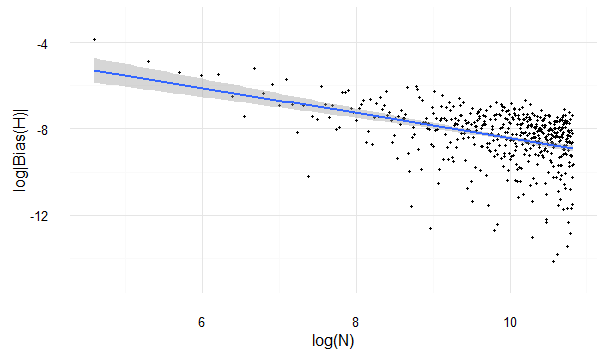
\includegraphics[width=\textwidth]{./Graphs/Best/Expo_k=2.png}
\caption{k=2}
\end{subfigure}%
\begin{subfigure}[b]{.8\textwidth}
\centering
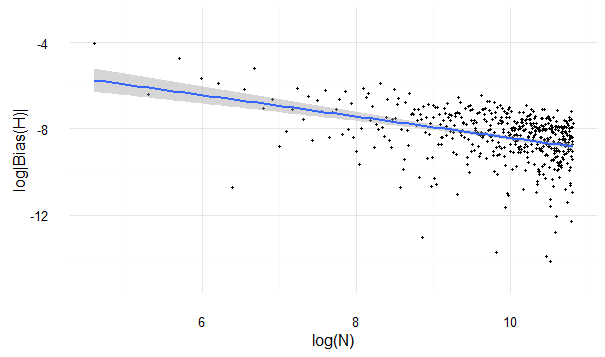
\includegraphics[width=\textwidth]{./Graphs/Best/Expo_k=3.png}
\caption{k=3}
\end{subfigure}%
}\    \makebox[\linewidth][c]{%
\begin{subfigure}[b]{.8\textwidth}
\centering
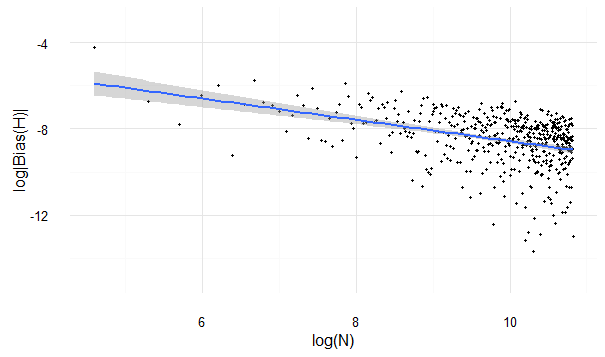
\includegraphics[width=\textwidth]{./Graphs/Best/Expo_k=4.png}
\caption{k=4}
\end{subfigure}%
\begin{subfigure}[b]{.8\textwidth}
\centering
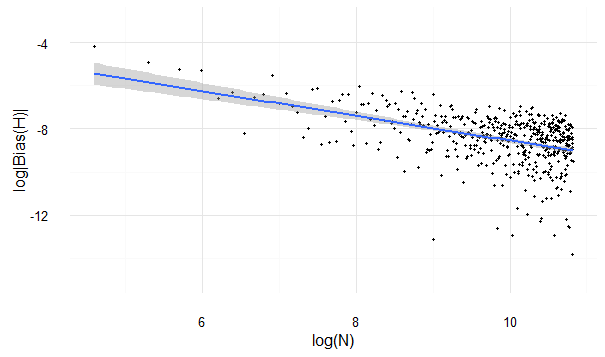
\includegraphics[width=\textwidth]{./Graphs/Best/Expo_k=5.png}
\caption{k=5}
\end{subfigure}%
}\    \makebox[\linewidth][c]{%
\begin{subfigure}[b]{.8\textwidth}
\centering
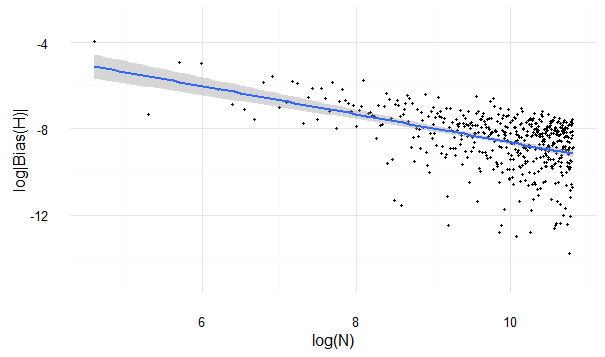
\includegraphics[width=\textwidth]{./Graphs/Best/Expo_k=6.png}
\caption{k=6}
\end{subfigure}%
}
\caption{1-dimensional Exponential distribution with different $k = 2, ..., 6$} \label{Expo_graphs26}
\end{figure}


\begin{figure}
\makebox[\linewidth][c]{%
\begin{subfigure}[b]{.8\textwidth}
\centering
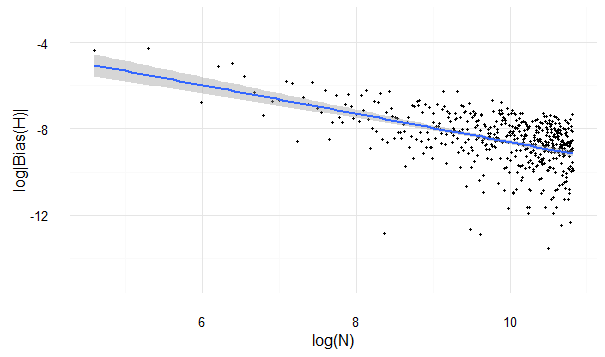
\includegraphics[width=\textwidth]{./Graphs/Best/Expo_k=7.png}
\caption{k=7}
\end{subfigure}%
\begin{subfigure}[b]{.8\textwidth}
\centering
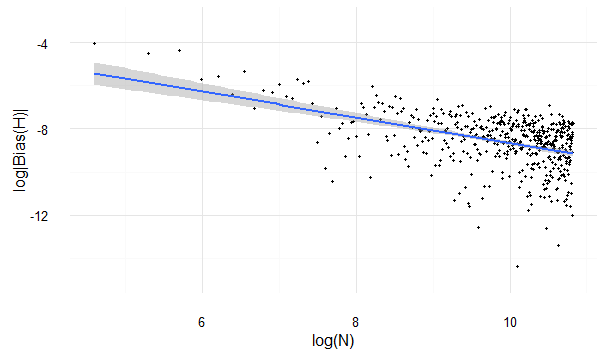
\includegraphics[width=\textwidth]{./Graphs/Best/Expo_k=8.png}
\caption{k=8}
\end{subfigure}%
}\    \makebox[\linewidth][c]{%
\begin{subfigure}[b]{.8\textwidth}
\centering
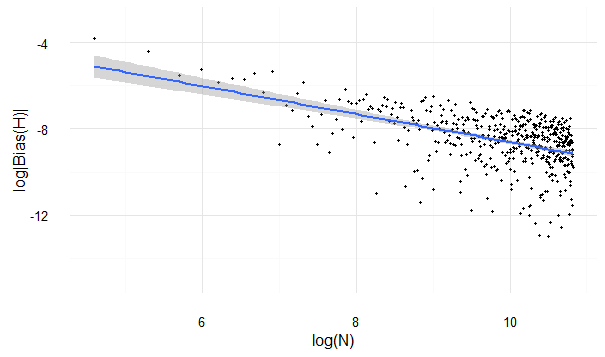
\includegraphics[width=\textwidth]{./Graphs/Best/Expo_k=9.png}
\caption{k=9}
\end{subfigure}%
\begin{subfigure}[b]{.8\textwidth}
\centering
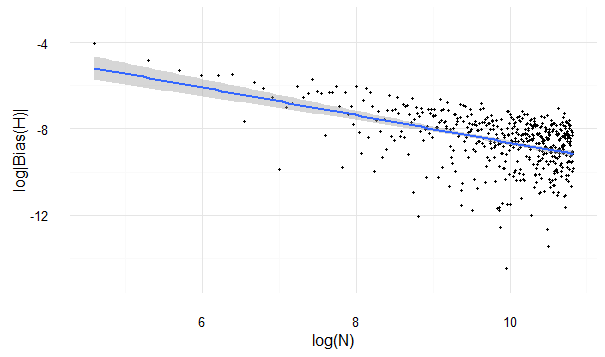
\includegraphics[width=\textwidth]{./Graphs/Best/Expo_k=10.png}
\caption{k=10}
\end{subfigure}%
}\    \makebox[\linewidth][c]{%
\begin{subfigure}[b]{.8\textwidth}
\centering
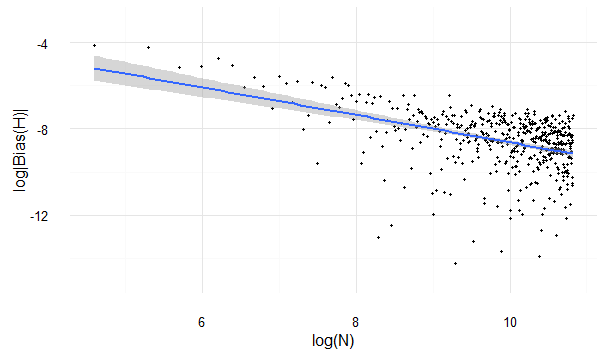
\includegraphics[width=\textwidth]{./Graphs/Best/Expo_k=11.png}
\caption{k=11}
\end{subfigure}%
}
\caption{1-dimensional Exponential distribution with different $k = 7, ..., 11 $} \label{Expo_graphs711}
\end{figure}

These graphs all show what we expected, and what has been confirmed with the previous two distributions, that the logarithm of the sample size against the logarithm of the bias of the estimator does indeed show a linear relationship. In these graphs there seems to be little difference between the values of $k$, in both the gradient of the line and in how close the data actually fits the line. This motivates us to consider both the coefficient of determination and the standard deviations of the regression for each value of $k$, which is given in Table \ref{expo_rsq}.

\begin{table}
\caption{Comparison of the coefficient of determination and the standard deviations of the regression for each value of $k$ for the 1-dimensional exponential distribution} \label{expo_rsq}
\begin{center}
\begin{tabular}{| l | c c |} 
\toprule
$k$ & $R^2$ & $\sigma$ \\
\midrule[1pt]
2     & 0.1843    & 1.1972   \\
3     & 0.1596    & 1.1073   \\
4     & 0.1538    & 1.1321   \\
5     & 0.2151    & 1.0687   \\
6     & 0.2277    & 1.1694   \\
7     & 0.2474    & 1.1253   \\
8     & 0.2107    & 1.1473   \\
9     & 0.2509    & 1.0939   \\
10    & 0.2200    & 1.2150   \\
11    & 0.2017    & 1.2369   \\
\hline
\end{tabular}
\\[10pt]
\end{center}
\end{table}

The $R^2$ value (coefficient of determination) is $\approx 0.207$, with very little variation, for all values of $k$. This is an indication that the regression line could be a poor fit to the data, since a value of 1 means a perfect fit. However, the standard error of the regression line is small, $\approx 1.15$ for all $k$, again with little variation. The standard error for the lines here is similar to that for both the uniform and normal distributions; thus, this doesn't necessarily indicate an extremely poorly fitting line.

The most important information found from these graphs is the equation of the regression line. I have collated all the data about the coefficients $a_{k}$ and $c_{k}$ and displayed them in Table \ref{expo_a_c_compare_table}.

\begin{table}
\caption{Comparison of coefficients of regression $a_{k}$ and $c_{k}$ from equation \ref{bias}, for 1-dimensional exponential distribution} \label{expo_a_c_compare_table}
\begin{center}
\begin{tabular}{| l | l l |} 
\toprule
$k$ &  $a_{k}$ & $c_{k}$ \\
\midrule[1pt]
2     & 0.5824    & 0.0739   \\
3     & 0.4941    & 0.0310   \\
4     & 0.4940    & 0.0266   \\
5     & 0.5727    & 0.0602   \\
6     & 0.6500    & 0.1199   \\
7     & 0.6605    & 0.1324   \\
8     & 0.6067    & 0.0739   \\
9     & 0.6480    & 0.1189   \\
10    & 0.6606    & 0.1267   \\
11    & 0.6365    & 0.1042   \\
\hline
\end{tabular}
\\[10pt]
\end{center}
\end{table}

This distribution shows interesting results, that are somewhat different to those previously shown in the other two distributions. In a similar fashion to previously there is a general increase in $a_{k}$ with $k$; however, in comparison to before where $c_{k}$ acted similarly, here $c_{k}$ does not increase uniformly with $k$. Both the values of $a_{k}$ and $c_{k}$ are unvaried between each $k$, with $a_{k}$ ranging from $0.4940$ to $0.6606$ and $c_{k}$ ranging from $0.0266$ to $0.1324$. Interestingly, the smallest values of $a_{k}$ and $c_{k}$, occur at $k=4$ then at $k=3$. Additionally, the largest two values occur at $k=7$ and $k=10$. The optimal value of $k$ will hopefully become more apparent when plotting all the regression lines against one and other in Figure \ref{expo_comparison_graph}.

Firstly, I wish to look at the relationship between $k$ and $c_{k}$ in the exponential distribution. To do this, I will look at the values of $c_{k}$ for each $k$ and see if it depends on $k^{a_{k}}$ or not. This should help us to decipher if the bias is of $O \left( \frac{1}{N^{a}} \right)$ or $O\left( \left( \frac{k}{N} \right)^{a} \right)$. This information is shown in table \ref{expo_dependentk}.

\begin{table}
\caption{Considering the dependence of $k$ on $c_{k}$} \label{expo_dependentk}
\begin{center}
\begin{tabular}{| l | l l l |} 
\toprule
$k$ &  $k^{a_{k}}$ & $c_{k}$ & $\frac{k^{a_{k}}}{c_{k}}$ \\
\midrule[1pt]
2     & 1.0000    & 0.0739    &    13.532   \\
3     & 1.4084    & 0.0310    &    45.434   \\
4     & 1.7207    & 0.0266    &    64.687   \\
5     & 2.2121    & 0.0602    &    36.745   \\
6     & 2.8466    & 0.1199    &    23.742   \\
7     & 3.2656    & 0.1324    &    24.665   \\
8     & 3.2563    & 0.0739    &    44.063   \\
9     & 3.8477    & 0.1189    &    32.361   \\
10    & 4.2695    & 0.1267    &    33.697   \\
11    & 4.3301    & 0.1042    &    41.556   \\
\hline
\end{tabular}
\\[10pt]
\end{center}
\end{table}

For the previous distributions there has been an obvious increase when looking at the values of $\frac{k^{a_{k}}}{c_{k}}$ for increasing $k$. However, for the exponential distribution this is not the case, the values seem to be all over the place, and plotting these in Figure \ref{c_k_expo} confirms this. 

\begin{figure}
\makebox[\linewidth][c]{%
\begin{subfigure}[b]{.8\textwidth}
\centering
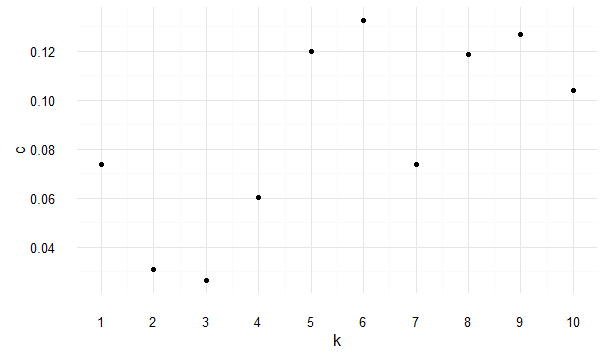
\includegraphics[width=\textwidth]{./Graphs/Best/ExpocVk.png}
\caption{The values of $k$ against the values of $c_{k}$}
\end{subfigure}%
\begin{subfigure}[b]{.8\textwidth}
\centering
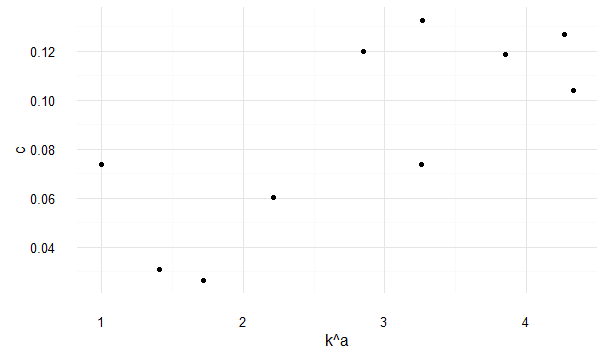
\includegraphics[width=\textwidth]{./Graphs/Best/ExpocVk2.png}
\caption{The values of $k^{a_{k}}$ against the corresponding values of $c_{k}$}
\end{subfigure}%
}
\caption{Graphically representing the relationship between $c_{k}$ and $k$ for the exponential distribution} \label{c_k_expo}
\end{figure}

These graphs do not show the almost exponential relationship seen before, they don't appear to show any relationship between $k$ and $c_{k}$. This could imply that for the exponential distribution we have $Bias| \hat{H}_{N, k} | = O \left( \frac{1}{N^{a}} \right)$, in comparison the normal and uniform which showed results in favour of the opposing idea;  $Bias| \hat{H}_{N, k} | = O\left( \left( \frac{k}{N} \right)^{a} \right)$.

To find the optimal value of $k$ for this distribution, I have generated a comparison plot of all of the regression lines, shown in Figure \ref{expo_comparison_graph}. Hopefully this can shed some light on which value of $k$ appears to be the best for use for the estimator, depending on the sample size $N$.

\begin{figure}
  \begin{center}
    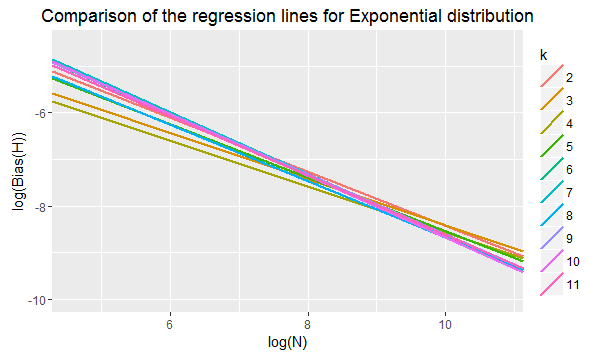
\includegraphics[width=\textwidth]{./Graphs/Best/ExpoComparison.png}
  \end{center}
\caption{Plot of regression lines for $\log|Bias(\hat{H}_{N, k})|$ against $\log(N)$, for $k=2, 3,..., 11$, for samples from the exponential distribution}
  \label{expo_comparison_graph}
\end{figure}

At smaller sample size $N \leq 5,000$, the graph appears to show that the estimator with $k=4$ has the lowest line; hence, the smallest bias and the best one to use for the estimation. However, for larger $N$ this is not true, to better visualise what is happening for large $N$, I have created an enlarged version in Figure \ref{expo_comparison_graph_zoom}.

\begin{figure}
  \begin{center}
    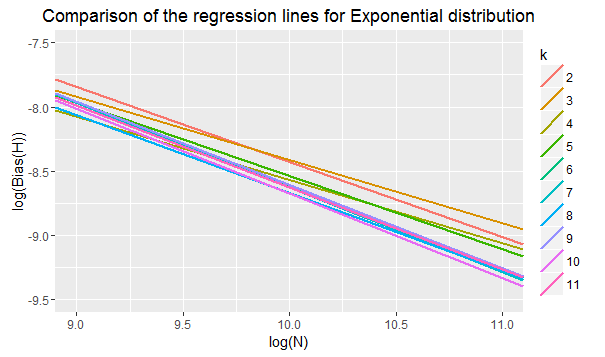
\includegraphics[width=\textwidth]{./Graphs/Best/ExpoComparisonZoom.png}
  \end{center}
\caption{Figure \ref{expo_comparison_graph} zoomed in around large $N$.}
  \label{expo_comparison_graph_zoom}
\end{figure}

This graph shows that for large sample sizes, $5,000 \leq N \leq 50,000$ that the estimator with $k=10$ has the smallest bias; thus appears to be the best one to use for estimating entropy from this distribution.









\chapter{Conclusion}

As seen from the analysis undertaken in Chapter \ref{Chapter_simulations}, taking an estimation of entropy from samples of the normal, uniform and exponential distributions, appear to act differently. There is no conclusive answer, that agrees across all three distributions,  as for the best value of $k$ for the estimator, or if the bias of the estimator is of $O \left( \frac{1}{N^{a}} \right)$ or $O\left( \left( \frac{k}{N} \right)^{a} \right)$. 

I previously discussed the supposed best value of $k$ as shown by the graphs with regression lines of the bias for each distribution. Where I mean optimal in terms of reducing the bias, so the estimated value is as close to the exact value as possible. To view this in more detail, comparing distributions and sample sizes, I have taken 1000 samples around the sample sizes of $500$, $10,000$, $20,000$, $30,000$, $40,000$ and $49,500$, found the average bias of the estimator for each $k$ and each distribution. I have graphically represented this in Figure \ref{OptimalK_graphs}. 

\begin{figure}
\makebox[\linewidth][c]{%
\begin{subfigure}[b]{.8\textwidth}
\centering
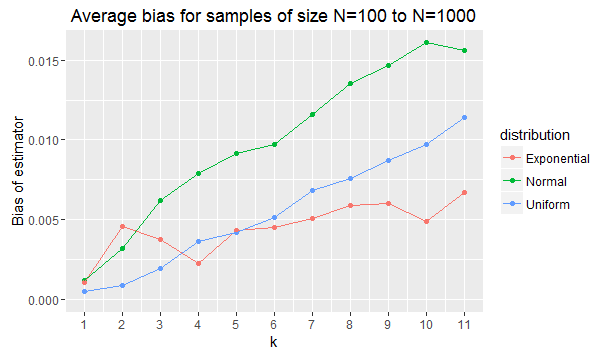
\includegraphics[width=\textwidth]{./Graphs/Best/kVbiasapprox100.png}
\caption{$N \approx 500$}
\end{subfigure}%
\begin{subfigure}[b]{.8\textwidth}
\centering
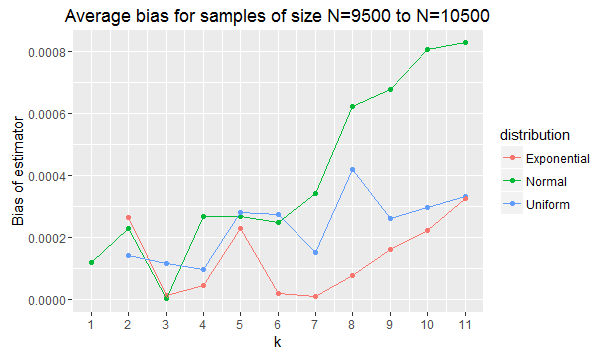
\includegraphics[width=\textwidth]{./Graphs/Best/kVbiasapprox10000.png}
\caption{$N \approx 10,000$}
\end{subfigure}%
}\    \makebox[\linewidth][c]{%
\begin{subfigure}[b]{.8\textwidth}
\centering
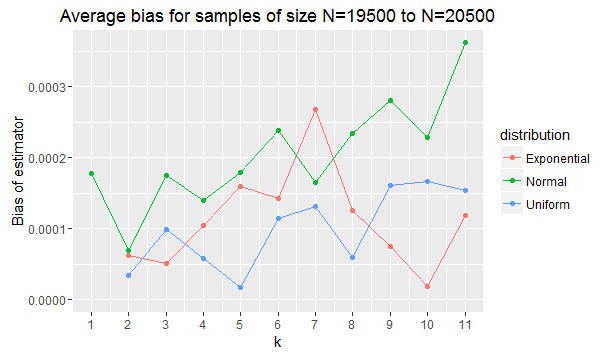
\includegraphics[width=\textwidth]{./Graphs/Best/kVbiasapprox20000.png}
\caption{$N \approx 20,000$}
\end{subfigure}%
\begin{subfigure}[b]{.8\textwidth}
\centering
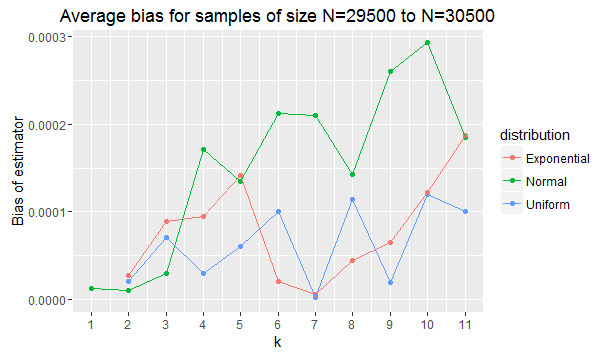
\includegraphics[width=\textwidth]{./Graphs/Best/kVbiasapprox30000.png}
\caption{$N \approx 30,000$}
\end{subfigure}%
}\    \makebox[\linewidth][c]{%
\begin{subfigure}[b]{.8\textwidth}
\centering
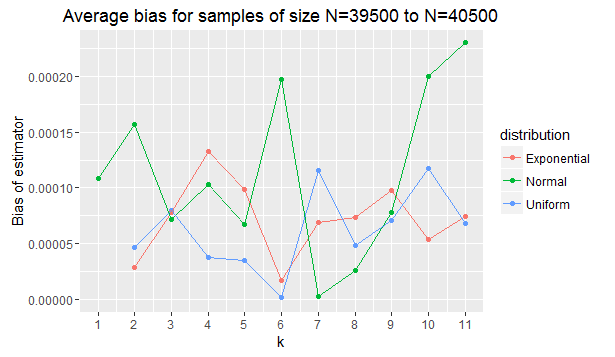
\includegraphics[width=\textwidth]{./Graphs/Best/kVbiasapprox40000.png}
\caption{$N \approx 40,000$}
\end{subfigure}%
\begin{subfigure}[b]{.8\textwidth}
\centering
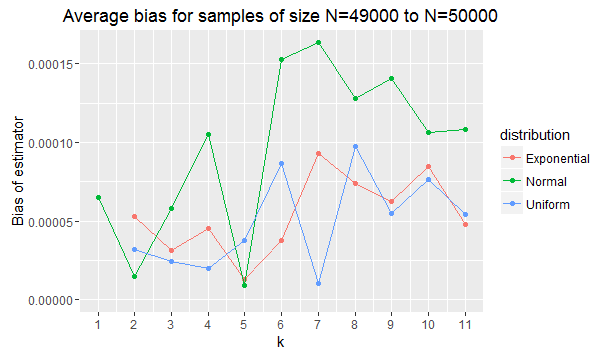
\includegraphics[width=\textwidth]{./Graphs/Best/kVbiasapprox50000.png}
\caption{$N \approx 49,500$}
\end{subfigure}%
}
\caption{Comparing the average bias about sample size $N$, for each $k$ and each distribution.} \label{OptimalK_graphs}
\end{figure}


If we ignore the distribution, there is not an always obvious best value of $k$ shown by the graphs. Moreover, considering the analysis completed in section \ref{N_conditions}, we found that the values of $k$ that satisfy Theorems \ref{unbias} and \ref{efficient}, depend on $N$ so that $k \in \{k_{0}^{*}, ..., k_{1}^{*}\}$, where $k_{0}^{*} \approx 1$ and $k_{1}^{*} = O(N^{\frac{2}{9}})$. Thus for the samples in the graphs above, we can create a table of the values of $k$ that satisfy the conditions to be able to assume consistency and unbias of the estimator, Table \ref{ConditionK}.

\begin{table}
\caption{Values of $k$ satisfying Theorems \ref{efficient} and \ref{unbias} for sample sizes $N$} \label{ConditionK}
\begin{center}
\begin{tabular}{| l | c |} 
\toprule
N &  $k$ \\
\midrule[1pt]
$500$ & $\{1, 2, 3\}$ \\
$1,000$ & $\{1,2, 3, 4 \}$ \\
$10,000$ & $\{1, 2, ..., 7\}$ \\
$20,000$ & $\{1, 2, ..., 9\}$ \\
$30,000$ & $\{1,2, ..., 9 \}$ \\
$40,000$ & $\{1, 2, ...,10 \}$ \\
$50,000$ & $\{1, 2,  ..., 11\}$ \\
\hline
\end{tabular}
\\[10pt]
\end{center}
\end{table}


Although, for samples of size $N \leq 1,000$, we can see that, quite obviously, the smallest bias occurs with an estimator found using $k=1$, and this is true for all the distributions, graph (a). If we consider the comparison graphs in Chapter \ref{Chapter_simulations}, when $N \leq 1,000$ we approximately have $log(N) \leq 7$, and in Figures \ref{normal_comparison_graph}, \ref{uniform_comparison_graph} and \ref{expo_comparison_graph} we have the lowest line, the smallest bias values at $k=2$, $k=3$ and $k=4$ for the normal, uniform and exponential samples respectively. This difference in results could be due to a number of reasons. Firstly, from the current analysis $k=1$ appears to be the optimal value for the smallest bias; however, when looking at the uniform and exponential samples, the regression line for $k=1$ was omitted, due to the large number of \texttt{Inf} values (reasoning for these values were discussed previously). Secondly, the graphs shown in Chapter \ref{Chapter_simulations} are of regression lines, which we have assumed to be linear as $N \to \infty$. Thus, when looking at the information shown by the lines in a particular region where $N$ is small, we cannot say that these are accurate. Therefore, the difference in results is not a problem; and the graph in Figure \ref{OptimalK_graphs} (a), is more accurate when looking at this $N$. Moreover, from this graph, we can see a uniform increase in the bias, against the size of $k$ for both the uniform and normal distributions; thus for $N \approx 500$ and $k \in \{1,2, 3\}$, the optimal estimator is definitely found using $k=1$. 


Considering graph (b) for sample size $N \approx 10,000$, we have that the smallest values of bias occur when $k=3$ or $7$ for the exponential, $k=3$ for the normal and $k=4$ for the uniform distributions. This agrees with the information found when finding $k$ to satisfy condition \ref{A3} we have that for this sample size $k \in \{1, 2, ... , 7\}$. This also implies that the most accurate estimator for a sample of this size could be found when using $k =3$ (or possibly $4$), since for all three distributions, at these values of $k$, we do have some of the smallest sizes of bias. When $N \approx 10,000$ we have $log(N) \approx 9.2$, which is where on Figures  \ref{normal_comparison_graph}, \ref{uniform_comparison_graph} and \ref{expo_comparison_graph}, the regression lines begin to cross. Thus, looking at these figures makes it difficult to decipher which value of $k$ appears to have the smallest bias, however, if we look at  Figures \ref{normal_comparison_graph_zoom}, \ref{uniform_comparison_graph_zoom} and \ref{expo_comparison_graph_zoom}, which zoom in around $log(N) \approx 9$, we can see that for the normal distribution, the lowest lines occur at $k=2$ then $3$, for the uniform $k=4$ then $3$ and for the exponential $k=8$ then $3$. The results in these graphs, as well as the graphs in this chapter all give the impression that $k=3$ is a strong choice for the optimal value of $k$ when finding the estimator for sample size $N \approx 10,000$.


For graph (c), with $N \approx 20,000$, we have a range of values for $k$ with the smallest bias, depending on the distribution; for the exponential $k=10$, the normal $k=2$ and uniform $k=5$. However, considering that for this sample size we must have $k \in \{1, 2, ..., 9\}$, the value of $k$ for the exponential distribution cannot be $k=10$ for the Theorems \ref{efficient} and \ref{unbias} to be satisfied; thus the next smallest bias occurs when $k=3$. Due to this, nothing conclusive can be said about the optimal value of $k$, although, we could draw the conclusion that for this sample size, the best $k$ is from the range $k = \{2, 3, 5\}$. However, when choosing the values of $k$ that satisfy condition \ref{A3}, I made some approximations, which depended on the choice of $\alpha > d = 1$, and a value $\tau$ which is smaller than a bound. Due to this, the value of $tau$ could be chosen to be slightly larger; for example $\tau = \frac{19}{80} < \frac{1}{4}$, which would give $k_{1}^{*} = N^{\frac{19}{80}} = 20000^{\frac{19}{80}} = 10.507$. So $k=10$ could be included in the values that satisfy the Theorems and cannot be discounted. In fact, if we did use this new value of $\tau$, then the values for the optimum $k$ would be $k = \{2, 5, 10\}$, which makes even less sense.

Moreover, we can also examine the graphs in Chapter \ref{Chapter_simulations}, for this sample size $N \approx 20,000$ which gives $log(N) \approx 9.9$. Thus, Figures \ref{normal_comparison_graph_zoom}, \ref{uniform_comparison_graph_zoom} and \ref{expo_comparison_graph_zoom}, which zoom around this sample size, show that the optimal choice of $k$ for the normal distribution is $k=5$, for the uniform is $k=7$ then $5$ and for the exponential $k=8$ or $10$. The exponential agrees on $k=10$ and the uniform agrees on $k=5$, but these are both the second lowest lines on the graph, and other that this non of the above results agree across distributions with those from earlier. This could be due to a number of reasons, but the most obvious one being that there is not a fixed value of $k$ for this sample size that coincides for all distributions as the optimal value of $k$. Thus, for this sample size we cannot draw any conclusions about the optimal value of $k$.


When $N \approx 30,000$, graph (d), we have the optimal values of $k$ - when the smallest bias occurs - being $2$ for the normal distribution and $7$ for both the uniform and exponential distributions. Interestingly, for all three distributions $k=2$ has either the first, second or third smallest bias, out of all $k$ for its own distribution. However, while the normal distribution has a general increase for $k > 2$, the other two distributions later dip to their lowest value of bias at $k=7$. Thus, while one may say that $k=7$ is the optimal, since it agrees with two of the three distributions, for the third distribution, the normal distribution, the bias is significantly higher. Henceforth, I would actually assume that a safer option, for the best value of $k$ across any distribution would be when $k=2$, where the bias for all three distributions is significantly small. Considering the regression lines, found in Chapter \ref{Chapter_simulations}, for $log(N) \approx 10.3$, we can see that the optimal choice of $k$ appears to be $k=5$ for the normal distribution, $k=8$ for the uniform and $k=10$ for the exponential. None of these agree with the possibility the $k=2$ is the optimal value, in fact when considering the graphs of the comparison of the regression lines for each distribution, we can see that the line for $k=2$ is not nearly the lowest of the group. More specifically for both the exponential and uniform distributions $k=2$ appears to be the worst possible value of $k$ in decreasing the bias, and since we are now considering a relatively large sample size, one would expect these graphs to have more accurate results. Although all these values of $k$ discussed fit within those found in Table \ref{ConditionK}; no value of $k$ stands out as an optimal value, thus no conclusion can be drawn for this sample size.


Now, for the graph (e), when $N \approx 40,000$ we have the smallest bias occurring at $k=6$ for the uniform and exponential and $k=7$ for the normal. If we consider the value for the bias at $k=6$ for the normal, we can see sudden significant increase in the size of the bias and a massive drop between this value, and that for $k=7$. Moreover, considering $k=7$ for the uniform and exponential distributions, we can see a substantial increase from the bias at $k=6$. Indicating, that the best value of $k$ may be $6$ or $7$; but this strongly depends on the distribution that the sample is taken from, not just the sample size. Now looking at the regression comparison graphs, around $N \approx 40,000$ we have $log(N) \approx 10.6$, which shows that for the normal distribution the optimal value of $k=5$ and $7$, for the uniform it's $k=7$ then $6, 8, 9$ (lines are very close) and for the exponential $k=10$ then $6, 7, 8$ (very close regression lines). This slightly agrees with above, that $k=6$ or $7$ could be the best value of $k$ to choose for the estimator; moreover, it also shows less of a dependence on distribution. Thus, I would suggest that for sample sized $N \approx 40,000$, that $k= \{6, 7\}$ would be the best candidates for the values of $k$.


Lastly, for the final graph (f) with sample size $N \approx 50,000$, we can see that instead of the uniform and exponential agreeing as before, we now have the normal and exponential agreeing on its minimum value of bias at $k=5$, and the uniform minimum occurring at $k=7$. For the uniform distribution, the estimator with $k=5$ still holds a small bias, but there are four other values of $k$ with smaller bias for this distribution. For the normal distribution, there is a large jump at $k=7$, where the bias is much larger than before, and the exponential also shows a substantial jump. For this sample size, we have $log(N) \approx 10.8$, so considering the enlarged regression graphs; Figures \ref{normal_comparison_graph_zoom}, \ref{uniform_comparison_graph_zoom} and \ref{expo_comparison_graph_zoom}, we can see that for each distribution the best value of $k$ in reducing the bias is given by $k=7$ then $5$ for the normal distribution, $k=7$ or $8$ for the uniform and $k=10$ for the exponential. Only the normal distribution aligns with above in that $k=7$ is the optimum value, but the rest does no coincide. However, both $k=5$ and $k=7$ appear in both analysis, a number of times so would be inclined to possibly agree that $k= \{5, 7\}$ are the optimal choices for this sample size $N \approx 50,000$, but this result is not certain for all distributions. 


By considering all the information found from the graphs in Figure \ref{OptimalK_graphs}, for small sample sizes $N \leq 1,000$ we can say that $k=1$ would possibly be the best choice for $k$. However, I don't think anything conclusive can be drawn about a general distribution from a larger sample size $N$, despite some of the rough deductions above, there is no definitive choice for $k$ being obviously shown throughout each distribution considered. 

Perhaps an interesting graph to look at is that depicted in Figure \ref{k_bias_allN}, where I have taken all the data for every sample size $100 \leq N \leq 50,000$ and averaged the bias per distribution. I have done this to see if there is a safer value of $k$ to choose when wanting the estimator of entropy from a random sample to have the smallest bias.

\begin{figure}
  \begin{center}
    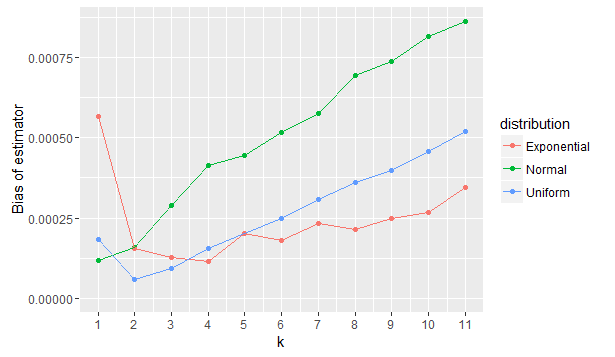
\includegraphics[width=\textwidth]{./Graphs/Best/kVbiasapproxALLN.png}
  \end{center}
\caption{The average bias over all sample sizes $N$ for each $k$ and each distribution.}
  \label{k_bias_allN}
\end{figure}

From this, we can see that for a sample distributed like the normal, the safest value of $k$ to choose for any sample size is $k=1$, since on average, this gives the smallest bias of $\approx 0.000125$, regardless of its sample size. Then for all other values of $k$, the bias of the estimator increases with $k$; hence, if in doubt, I would recommend choosing $k=1$ if you suspect your 1-dimensional data to be normally distributed.

Considering the uniform distribution, we can see that the smallest average bias occurs at $k=2$, with the same behaviour as the normal for $k \geq 3$, whereby the bias increases with $k$. The average bias at $k=2$ is $\approx 0.0000625$, which is about half the size of that for the normal distribution. However, even though the relative size of the bias within a distribution is important to look at, the size between distributions is not as informative, due to the variability of the samples. Where for the normal distribution we have variance $\sigma^2 = 1$ and for the uniform we have variance $\frac{12}{100^2} = 0.0012$, which is significantly smaller - so we would expect a more accurate estimator due to this. Thus, when uncertain of which $k$ to choose, if the 1-dimensional data appears to be uniformly distributed, then it seems to be that $k=2$ would be the best choice.

Lastly, looking at the most interesting result shown, those of the exponential distribution, which shows that, on average, the smallest bias occurs when $k=4$, with the bias generally increasing on both sides as $k$ increases/decreases away from $4$. The bias here is $\approx 0.000125$ - similar to that of the normal distribution, which is surprising owing to the fact that the samples from the exponential distribution were taken with a variability of $\frac{1}{0.5^2} = 4$, which is four times larger than the variance of the samples from the normal distribution. This is something very interesting about the exponential distribution, and I have noticed throughout my analysis that samples from this distribution do indeed act quite differently to those from the other two.

Another important aim of this paper was to consider whether the distributions imply the bias is of equations \ref{fixedkbias} or \ref{dependentkbias}; i.e, whether bias is of $O \left( \frac{1}{N^{a}} \right)$ or $O\left( \left( \frac{k}{N} \right)^{a} \right)$. From the previous section, namely Figures \ref{c_k_normal}, \ref{c_k_uniform} and \ref{c_k_expo}, implied the behaviours for the distributions considered shown in Table \ref{distribution_comparison}.

\begin{table}
\caption{Suspected behaviour of $Bias |\hat{H}_{N, k} |$ for each distribution} \label{distribution_comparison}
\begin{center}
\begin{tabular}{| c | c | c|} 
\toprule
Normal, $N(0,1)$ & Uniform, $U[0,100]$ & Exponential, $exp(0.5)$ \\
\midrule[1pt]
$O\left( \left( \frac{k}{N} \right)^{a} \right)$ & $O\left( \left( \frac{k}{N} \right)^{a} \right)$ &  $O \left( \frac{1}{N^{a}} \right)$ \\
\hline
\end{tabular}
\\[10pt]
\end{center}
\end{table}

This table shows that for samples from the normal and uniform distributions, both seemed to have the bias of the estimator showing the relation where $c_{k}$ depends on $k^a$, since the graphs of this correspondence, appeared to show an almost exponential relationship between the two variables. However, for the exponential distribution a very different picture occurred; thus, implying for this distribution that there was no obvious dependence on $k^a$, and in fact $c_{k}$ is just constant. 

Overall, this paper has shown that analytically, the estimator is asymptotically unbiased and that we cannot know how to choose $k$ for a sample by only considering its size $N$. We can only can find a range of $k$ that satisfies the conditions from the theoretical works, but the analytical results show that there are many discrepancies as to which value of $k$ is optimal, depending on how the sample is distributed. We have also not been able to draw any solid conclusions about the form of the bias of the estimator; however, the data here only showed implications of the connection between $c_{k}$ and $k^a$, it has not proved or disproved it either way.

There are large amounts of further research to be done into the estimation of entropy, but time permits that this paper can look at nothing more. With more time, it would be interesting to see how the estimator works analytically on samples from different distributions; for example, Gamma, Chi-Squared or Beta distributions. Also, it would be intriguing to look analytically at the estimator for samples from higher dimensions, with known entropy.






\begin{appendix}


\lstset{showstringspaces=false, breaklines=true}

\chapter{Code} \label{appendix_code}

For the simulations in this project, I used R; ''a language and environment for statistical computing and graphics'' \cite{code1}. I created a package called \texttt{EntropyEst}, with the functions needed to created the Kozachenko-Leonenko entropy estimator (KLEE). The functions exported form this package are; \texttt{KLEE}, \texttt{GammaFun}, \texttt{Rho}, \texttt{VolD}, \texttt{NormalEnt}, \texttt{UniformEnt}, \texttt{ExpoEnt} and \texttt{EntBias}. The functions in this package I then used to run simulations on samples from different statistical distributions to create the results in this paper.

To create my package \texttt{Entropy-Estimators}, I used two of Hadley Wickham's \cite{code2} packages; \texttt{devtools} and \texttt{roxygen2}. \texttt{Entropy-Estimators} also has only 1 dependent package (alongside the base R packages); \texttt{FNN}, which was used for the kth nearest neighbour function. 

When running simulations and creating the graphical information in this paper, I also used 5 more packages;  \texttt{ggplot2} for the graphical representation of the data, \texttt{Rcpp} to create a C++ for loop for faster computation, \texttt{dplyr} and \texttt{tidyr} for the manipulation of data, and \texttt{readr} to read and write the csv files of data.

I will outline the important code used for the simulations in this appendix; however, the full package and a complete account of the code used can be found on my GitHub page \textit{https://github.com/KarinaMarks/Entropy-Estimators}.

\section{The Estimator}

Using the definition of the Kozachenko-Leonenko estimator, found in Section \ref{focus}, I created the function \texttt{KLEE}. To do this I first had to make the following functions; \texttt{GammaFun}, \texttt{Rho}, \texttt{VolD}. For the purpose of this paper, I have only created the function to work out the estimator for a 1-dimensional sample.

Firstly, I created the function \texttt{Rho}, defined in equation \ref{Rho}, which takes three arguments;
\begin{itemize}
\item \texttt{X}; a vector of a sample to work out the distance between a value and its kth nearest neighbour
\item \texttt{k}; the order or nearest neighbour to be used
\item \texttt{d}; the dimension of the sample, default value 1 - since currently can only work for 1-dimensional samples
\end{itemize}
and returns a vector of distances, where its first entry is the distance from the first value of \texttt{X} to its kth nearest neighbour. The function is given by the following code;
\lstinputlisting[language=R]{./Code/Rho.R}

Next, I created the function \texttt{GammaFun}, defined in equation \ref{Gamma}, which takes one argument \texttt{m} and returns a numeric value, using the following code;
\lstinputlisting[language=R]{./Code/GammaFun.R}

Then, using the function above for $\Gamma$, we can define the function \texttt{VolD}, equation \ref{Volume}, which is the volume of the d-dimensional unit euclidean ball. This function takes one argument \texttt{d} which is the dimension and returns a numeric value using the following code;
\lstinputlisting[language=R]{./Code/VolD.R}

The only other function needed for the estimator is the digamma function which is defined in base R; thus, we can now define the estimator \texttt{KLEE}. This takes three arguments;
\begin{itemize}
\item \texttt{X}; a vector of a sample to estimate the entropy of
\item \texttt{k}; the order or nearest neighbour to be used
\item \texttt{d}; the dimension of the sample, default value 1 as before for \texttt{Rho}
\end{itemize}
and returns a numeric value which is the estimator of entropy for this distribution. The code written to define this function is as follows;
\lstinputlisting[language=R]{./Code/KLEE.R}


%\subsection{Example}
%To show that the \texttt{KLEE} function works, I am giving the example below where I can work out the estimation of entropy by hand, and check that my function works for this. 

%Consider a sample $X = \{3, 6, 1, 7, 2\}$, from this we can easily find the estimator of entropy for $k=1$ and $k=2$. For both estimators the sample szie $n=5$, the volume of the d-dimensional euclidean ball is $V_{d} = V_{1} = 2$. Then for $k=1$, the vector of nearest neighbour distances is given by $NN_{1} = \{1, 1, 1, 1, 1\}$ and the digamma function is given by $\Psi(1) = -\gamma \approx -0.57722$. Thus we have;

%\begin{align*}
%\hat{H}_{5, 1} (X) &= \frac{1}{5} \sum_{i=1}^{5} \frac{\log(NN_{1, i} \cdot 2 \cdot (5-1))}{\exp(-\gamma)} \\
%&=\frac{1}{5 \exp(-\gamma)} \sum_{i=1}^{5} \log(8) \\
%&= \frac{1}{\exp(-\gamma)} \log(8) \\
%&\approx something wrong
%\end{align*}

%For $k=2$ we have the vector of nearest neighbour distances is given by $NN_{2} = \{2, 3, 2, 4, 1\}$ and the digamma function is given by $\Psi(2) = -\gamma + 1 \approx 0.42278$. Thus we have;

%\begin{align*}
%\hat{H}_{5, 2} (X) &= \frac{1}{5} \sum_{i=1}^{5} \frac{\log(NN_{2, i} \cdot 2 \cdot (5-1))}{\exp(-\gamma + 1)} \\
%&=\frac{1}{5 \exp(-\gamma + 1)} \sum_{i=1}^{5} \log(8 NN_{2, i}) \\
%&= \frac{1}{5 \exp(-\gamma + 1)} \left(\log(16) + \log(24) + \log(16) + \log(32) + \log(8) \right)\\
%&\approx something? wrong
%\end{align*}


%TODO- look at both above?

%We can also find this using the function \texttt{KLEE}, by the following code;
%\begin{lstlisting}[language=R]
%> x <- c(3, 6, 1, 7, 2)
%> KLEE(x, k=1)
%[1] 2.656658
%> KLEE(x, k=2)
%[1] 2.430898
%\end{lstlisting}




\section{Exact Entropies}

To consider the bias of the estimator, I had to find the exact value of entropy from a 1-dimensional normal, uniform and exponential distribution. The function written to return this for the normal distribution is \texttt{NormalEnt} with parameter \texttt{sd}, the standard deviation of the sample, we do not need the mean value for finding the entropy of the normal distribution. The function is defined as follows;

\lstinputlisting[language=R]{./Code/NormalEnt.R}

With \texttt{sd =1}, as is true in the samples considered here, we find the entropy to be given by;

\begin{lstlisting}[language=R]
> NormalEnt(sd=1)
[1] 1.418939
\end{lstlisting}

The function for the uniform distribution is \texttt{UniformEnt}, with parameters \texttt{min} and \texttt{max}, is defined as;

\lstinputlisting[language=R]{./Code/UniformEnt.R}

Here we use \texttt{min=0} and \texttt{max=100} in the samples considered; thus we find the exact entropy to be given by;

\begin{lstlisting}[language=R]
> UniformEnt(min = 0, max = 100)
[1] 4.60517
\end{lstlisting}

Lastly, for the exponential distribution we have the function \texttt{ExpoEnt}, with only one parameter \texttt{rate}, defined below;

\lstinputlisting[language=R]{./Code/ExpoEnt.R}

In this paper we are using the exponential distribution with parameter \texttt{rate=1.5}, thus;

\begin{lstlisting}[language=R]
> ExpoEnt(rate = 1.5)
[1] 0.5945349
\end{lstlisting}



\section{Simulations}

\textit{In this section I used the packages \texttt{readr} to save the data, \texttt{dplyr} for the manipulation of data and \texttt{Rcpp} for creating a fast loop over hundreds of iterations.} 

I created functions \texttt{normalloop}, \texttt{uniformloop} and \texttt{expoloop}, in C++ which, for each sample size $N$ creates $M$ samples of that size, finds the estimator for sample and puts the result in a vector of length $M$. These functions are as follows;

\lstinputlisting[language=C++]{./Code/NormalLoop.R}

for the normal distribution, and for the uniform distribution;

\lstinputlisting[language=C++]{./Code/UniformLoop.R}

Lastly for the exponential distribution;

\lstinputlisting[language=C++]{./Code/ExpoLoop.R}

Using these functions I created each column of the tables, where each table is a different distribution, each column is a different value of $k \in \{1, 2, ..., 11\}$ and each row is a different sample size $N \in \{100, 200, 300, ..., 50000\}$. Below is how the column with $k=1$ for the normal distribution was created, all other columns were done similarly;

\lstinputlisting[language=R]{./Code/ColumnOfData.R}



\section{Analysis}

\textit{In this section I use the packages \texttt{ggplot2} for the graphs, \texttt{dplyr} for the data manipulation and \texttt{readr} to read in my csv data files.}

Once I obtained all the simulated data, I found the modulus of the bias for each sample size $N$, each $k$ and each distribution. I then selected the information for all $k$ with $N=100, 25000$ and $50000$, to display in Tables \ref{normal_kcompare_table}, \ref{uniform_kcompare_table} and \ref{expo_kcompare_table}, this involved taking \texttt{Data} and subtracting either \texttt{NormalEnt(sd=1)}, \texttt{UniformEnt(min=0, max=100)} or \texttt{ExpoEnt(rate=0.5)} from the estimators, depending on the distribution.

Next, I plotted graphs for each $k$ of the logarithm of the bias of the estimator $\hat{H}_{N, k}$ against the logarithm of the sample size $N$, shown in Figures \ref{normal_graphs16}, \ref{normal_graphs711}, \ref{Uniform_graphs26}, \ref{Uniform_graphs711}, \ref{Expo_graphs26} and \ref{Expo_graphs711}. I used the following code to do this, changing the \texttt{y} value to either \texttt{k1, k2, ..., k11} depending on which value of $k$ I was plotting. Also the \texttt{data} would be read in from a different file for each distribution, the code below shows plotting the simulations from the normal distribution with $k=1$.

\lstinputlisting[language=R]{./Code/logGraphEachK.R}

Additionally, I created a summary table of the useful information needed, containing the coefficients of the intercept $\zeta$ and the gradient $-a_{k}$ from the regression analysis, the coefficient of determination $R^2$ and the standard error $\sigma$ also from the regression analysis. I also modified $\zeta$ and$-a_{k}$ to find both $a_{k}$ and $c_{k}$. The code below shows how I did this for the normal distribution, and it is similar for the other two distributions, just changing the data inputted and the exact value of entropy used to find the bias.

\lstinputlisting[language=R]{./Code/SummaryTables.R}

These tables are shown in Appendix \ref{appendix_data}, and from these I found the information in Tables \ref{normal_rsq}, \ref{normal_a_c_compare_table}, \ref{uniform_rsq}, \ref{uniform_a_c_compare_table}, \ref{expo_rsq} and \ref{expo_a_c_compare_table}. Then to create Tables \ref{normal_dependentk}, \ref{uniform_dependentk} and \ref{expo_dependentk}, I just had to modify the summary tables found above to include two extra columns with the $k^{a_{k}}$ and $\frac{k^{a_{k}}}{c_{k}}$, which was done by the following;

\lstinputlisting[language=R]{./Code/Findingktoa.R}

From this table I than created the graphs shown in Figures \ref{c_k_normal}, \ref{c_k_uniform} and \ref{c_k_expo}, using the below code.

\lstinputlisting[language=R]{./Code/cVkGraphs.R}

The last part of analysis conducted, was plotting all the regression lines of the logarithm of $N$ against the logarithm of the bias, for each $k$ on the same graph. To do this I used the summary data, read in as \texttt{Info}, and the \texttt{xmin}, \texttt{xmax}, \texttt{ymin} and \texttt{ymax} found when plotting the graphs for each $k$ separately. The following code was then used to create the graphs in Figures \ref{normal_comparison_graph}, \ref{uniform_comparison_graph} and \ref{expo_comparison_graph};

\lstinputlisting[language=R]{./Code/ComparisonGraphs.R}



\section{Conclusion}

TODO - Talk about how I made the other graphs 



\chapter{Data} \label{appendix_data}

For all the data from the simulations visit \url{https://github.com/KarinaMarks/Entropy-Estimators/blob/master/Data/data_normal.csv} for the normal distribution, \url{https://github.com/KarinaMarks/Entropy-Estimators/blob/master/Data/data_uniform.csv} for the uniform distribution and \url{https://github.com/KarinaMarks/Entropy-Estimators/blob/master/Data/data_expo.csv} for the exponential distribution.

The data included here is the summary data created from the above simulated data, by the code set out in appendix \ref{appendix_code}. Note that for the uniform and exponential tables, there is no data for $k=1$, the reasons for this are set out previously in the appropriate chapters.

\section*{Simulations of Samples from the Normal Distribution - Summary Data}
    \begin{tabular}{c | c c c c c c}%
    $k$ & $a_{k}$ & $\zeta$ & $c_{k}$ & $R^2$ & $\sigma$
    \csvreader[head to column names]{normal.csv}{}
    {\\\hline\k & \a & \zeta & \c & \rsquared & \se}
    \end{tabular}

\section*{Simulations of Samples from the Uniform Distribution - Summary Data}
    \begin{tabular}{c | c c c c c c}%
    $k$ & $a_{k}$ & $\zeta$ & $c_{k}$ & $R^2$ & $\sigma$
    \csvreader[head to column names]{uniform.csv}{}
    {\\\hline\k & \a & \zeta & \c & \rsquared & \se}
    \end{tabular}

\section*{Simulations of Samples from the Exponential Distribution - Summary Data}
    \begin{tabular}{c | c c c c c c}%
    $k$ & $a_{k}$ & $\zeta$ & $c_{k}$ & $R^2$ & $\sigma$
    \csvreader[head to column names]{expo.csv}{}
    {\\\hline\k & \a & \zeta & \c & \rsquared & \se}
    \end{tabular}




\end{appendix}



\bibliographystyle{plain}
\bibliography{Bibliography}




\end{document}